% !TEX TS-program = latex
% !TEX TS-program = xelatex
% -*- mode : latex; coding: utf-8 -*-

%% 재단 맡길 때에는 showtrims을 켜서 a4로 출력 후 잘라내면 됨.
% \documentclass[11pt,a4paper,oneside,openany,reqno,chapter,nokorean,showtrims]{oblivoir}
\documentclass[11pt,a4paper,oneside, openany, reqno, chapter, nokorean]{oblivoir}
\setstocksize{297mm}{210mm}
% \settrimmedsize{\stockheight}{\stockwidth}{*}

%\usepackage[utf8]{inputenc}
\usepackage[dbl4x6]{fapapersize}
\usepackage{fapapersize}
\usefapapersize{210mm,297mm,40mm,30mm,30mm,32mm}

%% figure setting
% \usepackage{geometry}

\usepackage{textcomp}

\usepackage{pgfplots}
\pgfplotsset{width=7cm, compat=1.16}


\let\interHchar\undefined
\let\interhword\undefined
\usepackage[default]{dhucs-interword}
% \usepackage{dhucs-gremph}
\usepackage{dhucs-enumerate}
\usepackage{ifpdf}
\usepackage{url}
\usepackage{rotating}
\usepackage{titletoc}
\usepackage{titlesec}
% \usepackage[toc,page,header]{appendix}
% center the toc heading
% \titleformat{\chapter}[display] {\normalfont\bfseries}{}{0pt}{\Huge}
\titleformat{\chapter}[display]
  {\normalfont\bfseries}{}{0pt}{\Huge}

%\usepackage{cleveref}

% Define formats

\usepackage{lipsum} 

\newcommand{\BibTeX}{\textsc{Bib}\TeX}

\chapterstyle{default}
\usepackage{titletoc}% http://ctan.org/pkg/tocloft
\def\cftchapteraftersnum{.}
\renewcommand{\cftchapterdotsep}{\cftdotsep}% Chapters should use dots in ToC

\makeatletter
\def\@makechapterhead#1{%
  %%%%\vspace*{50\p@}% %%% removed!
  {\parindent \z@ \raggedright \normalfont
    \ifnum \c@secnumdepth >\m@ne
        % \huge\bfseries \@chapapp\space \thechapter
        \par\nobreak
        \vskip 20\p@
    \fi
    \interlinepenalty\@M
    \LARGE \bfseries \thechapter. #1\par\nobreak
    \vskip 20\p@
  }}
\def\@makeschapterhead#1{%
  %%%%%\vspace*{50\p@}% %%% removed!
  {\parindent \z@ \raggedright
    \normalfont
    \interlinepenalty\@M
    \LARGE \bfseries  #1\par\nobreak
    \vskip 40\p@
  }}
\makeatother

\ifpdf

\hypersetup{
colorlinks = true
} 
\fi

\usepackage{amsmath,amsthm,amssymb,amsxtra}
\usepackage{graphicx}
\newsubfloat{figure}
\usepackage{epsfig}
\let\footruleskip\undefined
\usepackage{fancyhdr}
\usepackage{environ}
\usepackage{siunitx}
\ifpdf
% enable hyper links
\hypersetup{
 pdftitle={Thesis},
 pdfauthor={Author name},
 pdfkeywords={j/psi,charmed meson},
 citecolor=black,
 %citecolor=darkblue,
 filecolor=black,
 linkcolor=black,
 %inkcolor=darkblue,
 urlcolor=blue,
 colorlinks=true}
\fi
\usepackage{seoultech} % 서울과학기술대학교 양식

\setlength\parindent{2pc} % 들여쓰기 1글자

\newtheorem{theorem}{Theorem}[chapter] % Theorem 1.1, Theorem 3.4
\newtheorem{corollary}[theorem]{Corollary} % Corollary는 독자번호 없음.
\newtheorem{lemma}[theorem]{Lemma}
\newtheorem{proposition}[theorem]{Proposition}
\newtheorem{question}{Question} % 독자적인 번호를 갖는다. Question 1, Question 2
\newtheorem{step}{Step}

% 번호를 붙이지 않는 `정리' 만들기
\newtheorem{lemmawon}{Lemma}
\newtheorem{claim}{Claim}

% 특별한 이름을 갖는, 번호가 붙지 않는 Theorem 만들기
\newtheorem{questionA}{Question~A}
\newtheorem{mainthmA}{Main Theorem~A}

% 본문의 글씨가 기울어지지 않는 환경
\theoremstyle{definition}
\newtheorem{definition}[theorem]{Definition}

% 화면에 나오는 이름이 이탤릭체인 환경
\theoremstyle{remark}
\newtheorem{remark}[theorem]{Remark}
\newtheorem{remarkof}{Remark}[theorem] % 어떤 Theorem의 아래에 Remark
\newtheorem{remarkwon}{Remark}

% 수식 번호 붙이기 (1.1), (3.3)
\numberwithin{equation}{chapter} 

%책갈피용
%\usepackage[bookmarks=true]{hyperref}
\usepackage{bookmark}


\setcounter{secnumdepth}{4}
\setcounter{tocdepth}{2}


%표 정렬용
\usepackage{multirow}
\renewcommand{\multirowsetup}{\centering}

%그림위 글자 기능(인준서 도장용)
\usepackage[abs]{overpic}
\setlength\unitlength{1mm}

\usepackage{setspace}
%\doublespacing
\usepackage{array}
\usepackage{makecell}
\usepackage{multirow}
\usepackage{parallel,enumitem}
\usepackage{graphicx}
\usepackage{tikz}
\usetikzlibrary{shapes,decorations.pathmorphing}
\usepackage{amssymb}% http://ctan.org/pkg/amssymb
\usepackage{booktabs}
% \usepackage{adjustbox}
\usepackage{amsmath}
\usepackage{algorithm}
\usepackage{algorithmicx}
\usepackage[noend]{algpseudocode}
\usepackage[flushleft]{threeparttable}

\usepackage{subcaption}
\usepackage{siunitx}
\usepackage{tabularx}
\usepackage{enumitem}

\usepackage{amsthm}
\usepackage{stmaryrd}
\usepackage{amsfonts}
\usepackage{xcolor}

\usepackage{array}
\newcolumntype{L}[1]{>{\raggedright\let\newline\\\arraybackslash\hspace{0pt}}m{#1}}
\newcolumntype{C}[1]{>{\centering\let\newline\\\arraybackslash\hspace{0pt}}m{#1}}
\newcolumntype{R}[1]{>{\raggedleft\let\newline\\\arraybackslash\hspace{0pt}}m{#1}}

\usepackage{fontspec}
\newfontfamily\unbatang{UnBatang.ttf}
\usepackage{kotex}

% \setmainfont{Times New Roman}
% \setsansfont{Arial}
% \setmonofont{Courier New}

%%%%%%%%%%%%%%%%%%%%%%%%%%%%%%%%%%%%%%%%%%%%%%%%%%%%%%%%%%%%%%%%%%%%%%%%%%%
% to be able to draw some self-contained figs
\usepackage{tikz}
\usepackage{amsmath}
%%%%%%%%%%%%%%%%%%%%%%%%%%%%%%%%
% inlined bib file

%%%%%%%%%%%%%%%%%%%%%%%%%%%%%%%%%%%%%
\newcommand{\minus}{\scalebox{0.75}[1.0]{$-$}}
\theoremstyle{definition}
\theoremstyle{remark}
\theoremstyle{definition}

\algnewcommand\algorithmicinput{\textbf{Input:}}
\algnewcommand\INPUT{\item[\algorithmicinput]}
\algnewcommand\algorithmicoutput{\textbf{Output:}}
\algnewcommand\OUTPUT{\item[\algorithmicoutput]}

%%%%%%%%%%%%%%%%%%%%%%%%%%%%%%%%%%%%%%%%%%%%%%%%%%%%%%%%%%%%%%%%%%%%%%%%%%%%%%



\DeclareMathOperator*{\argmax}{argmax} % thin space, limits underneath in displays
  
\begin{document}
  %% 정보
  \EnglishTitle{Feature-Aware Numerical Representation for Retrieval-Augmented Medical Tabular Classification (FiTabr)}
  %% 본문이 영문일 경우, 국문 제목은 빈칸으로 둘 것
  \KoreanTitle{}
  \AuthorKoreanName{저자 한국 이름}
  \AuthorEnglishName{Kurbanov Elvin Vagibovich}
  \KoreanNameofDegree{공학 석사}
  
  \EnglishNameofDegree{Master of Science}
  \EnglishNameofPaper{Master Thesis}

  \GraduateDate{2026년 2월}
  \GraduateDateEnglish{February 2026}
  \EnglishDepartmentName{Department of Computer Science and Engineering}
  \KoreanDepartmentName{학과 한글 이름}
  \RefereeChief{심사위원장 이름}
  \RefereeSecond{심사위원1 이름}
  \RefereeThird{심사위원2 이름}
  \AdvisorKoreanName{지도교수 한글 이름}
  \AdvisorEnglishName{Taesoo Kwon}

%% 앞표지
\makefrontcover


%% 
\englishproposal

%% 국문 제출 승인서. 국문 인준서의 경우 업데이트가 되지 않아서 추가 작업 필요.
%\makeapproval

%% 영문 제출 승인서
\makeenglishapproval

\pagenumbering{gobble}


\cedp
  
 %% 본문 이전의 쪽들
\frontmatter 


\phantomsection
\addcontentsline{toc}{chapter}{Summary}
\markboth{Summary}{}
\begin{EnglishSummary}
With the increasing application of artificial intelligence in healthcare, medical tabular data have become an important source for clinical prediction tasks. Such datasets typically combine heterogeneous patient-related variables, including demographic characteristics, laboratory measurements, and physiological indicators. Often these variables differ in type, scale, have class-imbalanced, how informative each variable is for prediction and clinical datasets are mostly small, which makes learning challenging. Retrieval-based tabular methods address this by using similar training samples during prediction. In particular, ModernNCA achieves strong results by learning a feature transformation before neighbor retrieval, suggesting that feature weighting before retrieval affects performance. This thesis therefore proposes FiTabR, a feature-aware extension of the retrieval-augmented model TabR. FiTabR adds a lightweight attention module before the TabR encoder that generates sample-specific weights for numerical features and applies residual feature modulation, while preserving TabR's retrieval and prediction mechanisms. Across three medical datasets, FiTabR improves on TabR only under certain conditions. On Heart Disease, accuracy increases from 0.8841 to 0.8937 and cross-entropy decreases from 0.3586 to 0.3038. On Pima Diabetes, the gain is small (0.7529 to 0.7586), and on Stroke Prediction both models reach identical accuracy, with FiTabR showing a slightly lower ROC-AUC (0.8095 versus 0.8136). On Heart Disease, ablation shows that removing residual preservation reduces accuracy to 0.8647 and uniform weighting increases cross-entropy to 0.3240, whereas removing attention scaling does not reduce performance. Attention analysis on the same dataset assigns the highest weights to cholesterol and age, consistent with cardiovascular knowledge, but the lowest to exercise-induced ST-segment depression and maximum heart rate despite their prognostic value. These findings indicate that the benefit of feature-aware representation in retrieval-augmented learning is dataset dependent.



\end{EnglishSummary}

    
\pagenumbering{gobble}
 
    

\cedp
  
  %% 본문 이전의 쪽들
\frontmatter 

  %% TOC/ LOF / LOT 끝의 * 지우면 안됨. ( 목차에서 명단 삭제 필요 )

\pagestyle{plain}%
	%% 목차
\clearpage
\phantomsection 
\renewcommand{\contentsname}{Table of Contents}
\setcounter{tocdepth}{1}
\tableofcontents*
    %% 표목차

\clearpage
\phantomsection
\listoftables*
\addcontentsline{toc}{chapter}{List of Tables}

\clearpage
\phantomsection
\listoffigures*
\addcontentsline{toc}{chapter}{List of Figures}
        
  %%% 본문 시작
  \mainmatter
  \linespread{2}
  %\SetHangulspace{2.2}{2.0}

  %% 쪽번호가 아래 중앙에 붙는다.
  % \pagestyle{fancy}%
  % \lhead{\leftmark}%
  % \rhead{}%
  % \chead{}%
  \cfoot{\thepage}%
  \renewcommand{\headrulewidth}{0pt}

    \chapter{Introduction}

Machine learning has become increasingly relevant to medical prediction as
clinical information is progressively collected and stored in structured
digital form. Many clinical prediction problems are naturally represented as
tabular data composed of demographic characteristics, physiological
measurements, laboratory values, medical history, and other patient-related
variables. Such data support a wide range of predictive tasks, including
disease identification, risk estimation, and clinical outcome prediction
\cite{rajkomar2019mlmedicine}. However, medical tabular data also present
several challenges for predictive modeling. Compared with the large-scale
datasets commonly available in computer vision and natural language processing,
medical datasets are often relatively small, may contain heterogeneous feature
types, and can exhibit substantial differences in class distribution and
predictive structure across clinical tasks.

Traditional machine learning methods, particularly tree-based models, remain
strong approaches for tabular prediction. Gradient-boosted decision trees such
as XGBoost, LightGBM, and CatBoost have demonstrated competitive performance
across a wide range of structured-data problems
\cite{chen2016xgboost,ke2017lightgbm,prokhorenkova2018catboost}. In contrast,
the advantages of deep learning on conventional tabular datasets have been less
consistent than in image, text, and speech applications. Previous studies have
shown that carefully tuned tree-based models frequently remain competitive with
or outperform deep neural networks on typical tabular benchmarks
\cite{grinsztajn2022tree}. Nevertheless, recent advances in tabular deep
learning have introduced architectures designed specifically to improve the
representation of numerical and categorical variables and to model interactions
between features and observations
\cite{gorishniy2021revisiting,gorishniy2022embeddings,somepalli2021saint}.

One important direction within this development is retrieval-augmented tabular
learning. Rather than generating a prediction solely from parameters learned
during training, retrieval-augmented models additionally use information from
relevant observations stored in the training set. For a given target sample,
similar observations are retrieved and incorporated into the prediction
process. This idea connects representation learning with local information from
the available data and has motivated several retrieval-based approaches for
tabular prediction
\cite{qin2021rim,kossen2021selfattention,gorishniy2024tabr}.

TabR is a recent retrieval-augmented deep learning model for tabular data that
combines a feed-forward architecture with a nearest-neighbor-like retrieval
mechanism \cite{gorishniy2024tabr}. The model first constructs a learned
representation of the target observation and candidate training observations.
Candidate samples are then retrieved according to similarity in the learned
representation space, and information from the retrieved observations is
incorporated through a contextual aggregation mechanism before the final
prediction is produced. TabR demonstrated that an appropriately designed
retrieval mechanism can substantially improve the competitiveness of deep
learning for tabular prediction. At the same time, the original TabR study
also showed that retrieval is not uniformly beneficial for every dataset,
highlighting the importance of dataset characteristics in determining the
effectiveness of retrieval-based learning.

The behavior of a retrieval-augmented model depends not only on how candidate
observations are retrieved, but also on the representation from which
similarity is determined. In TabR, numerical and categorical inputs are encoded
into learned sample representations before candidate retrieval is performed.
The retrieval component therefore operates on representations whose geometry
depends on how the original input variables are transformed. However, the
original TabR architecture does not explicitly introduce sample-specific
reweighting of individual numerical variables before the encoder. Its
specialized attention-like mechanism is instead primarily associated with the
retrieval and aggregation of candidate observations.

This distinction motivates the central question investigated in this thesis.
Medical tabular datasets commonly contain numerical measurements whose
predictive relevance may vary across prediction tasks and individual samples.
An explicit mechanism that allows the numerical representation to adapt to the
characteristics of each observation may therefore influence the representation
subsequently used by the retrieval model. At the same time, modern neural
networks are already capable of learning nonlinear transformations of their
inputs, and it cannot be assumed in advance that an additional feature-aware
mechanism will consistently improve predictive performance. The effect of such
a modification must therefore be evaluated empirically and separated from
changes to the retrieval architecture itself.

To investigate this problem, this thesis proposes \textit{FiTabR}, a
feature-aware extension of TabR for medical tabular classification. FiTabR
introduces a lightweight attention network that operates on numerical features
before the TabR encoder. For each input sample, the attention module produces
a distribution over the numerical variables. These values are then used to
modulate the numerical input through residual feature reweighting. The
resulting representation is subsequently processed by the original TabR
encoder and retrieval pipeline.

For a numerical feature vector $\mathbf{x}_i$, the FiTabR representation is
defined as

\begin{equation}
    \tilde{\mathbf{x}}_i
    =
    \mathbf{x}_i
    \odot
    \left(
        1 + \alpha \mathbf{a}_i
    \right),
    \label{eq:fitabr_intro}
\end{equation}

where $\mathbf{a}_i$ denotes the sample-specific attention distribution,
$\alpha$ is the attention scaling coefficient, and $\odot$ denotes
element-wise multiplication. The residual term preserves the original
numerical input while allowing the learned attention mechanism to modify its
magnitude before encoding. Importantly, FiTabR does not replace the retrieval
mechanism of TabR. Candidate retrieval, contextual aggregation, and the final
prediction mechanism are retained. The architectural change is therefore
localized to the numerical representation supplied to the TabR encoder.

This controlled design makes it possible to examine whether changes in
pre-retrieval numerical representation can affect the behavior of a
retrieval-augmented model without simultaneously redesigning its retrieval
mechanism. Accordingly, the primary research question of this thesis is:

\begin{quote}
\textit{Can sample-specific numerical feature modulation provide useful
improvements to retrieval-augmented tabular classification while preserving
the underlying TabR retrieval framework?}
\end{quote}

Two additional questions follow from this objective. First, if differences in
performance are observed, which components of the proposed representation
mechanism are responsible for them? Second, does the learned feature-attention
mechanism provide meaningful information about how the model emphasizes
numerical clinical variables across different observations?

To address these questions, FiTabR is evaluated on three medical binary
classification tasks: Heart Disease, Pima Diabetes, and Stroke Prediction.
These datasets provide different experimental conditions in terms of sample
size, feature composition, and class distribution. FiTabR is compared directly
with the original TabR architecture and with conventional machine learning and
deep tabular learning baselines. The purpose of the cross-dataset evaluation
is not to assume that feature-aware representation will improve every medical
prediction task, but to determine whether its effect is consistent and to
identify the conditions under which the proposed mechanism is beneficial.

The experimental findings provide partial rather than universal support for
the initial hypothesis. FiTabR shows its clearest improvement relative to TabR
on the Heart Disease dataset, whereas the differences observed on Pima Diabetes
are more modest. On the severely imbalanced Stroke Prediction dataset, the
proposed representation mechanism does not improve threshold-based
minority-class prediction. These results indicate that explicit feature-aware
numerical representation can influence retrieval-augmented tabular learning,
but that its effectiveness depends on the characteristics of the underlying
dataset. In particular, modifying feature representation alone is not
sufficient to address learning problems dominated by severe class imbalance.

Predictive comparison between TabR and FiTabR alone is insufficient to
determine why the proposed method behaves differently. For this reason, the
thesis additionally conducts a component-level ablation study. Three
architectural variants are examined: a model without residual feature
preservation, a model without the explicit attention-scaling factor, and a
model in which learned feature attention is replaced by uniform weighting.
These experiments distinguish the contribution of residual preservation,
numerical modulation, and sample-specific nonuniform weighting. The ablation
results show that the components do not contribute equally across datasets.
Residual feature preservation receives the clearest empirical support,
particularly on Heart Disease, whereas fixed attention scaling and learned
nonuniform feature weighting exhibit more dataset-dependent effects.

The feature-attention mechanism also provides an explicit internal signal that
can be examined independently of overall predictive performance. Attention
values are therefore analyzed across samples using their mean and standard
deviation. The mean attention assigned to a feature describes its average
model-assigned emphasis across the dataset, while the standard deviation
characterizes how strongly this emphasis varies between individual samples.
These patterns are compared with established medical domain knowledge to
examine whether the representation learned by FiTabR exhibits clinically
plausible correspondence. Attention-based tabular models have previously been
used to expose feature-selection and interaction behavior
\cite{arik2021tabnet}; however, attention values should not automatically be
interpreted as causal explanations. Accordingly, the analysis in this thesis
treats FiTabR attention as evidence of internal model behavior rather than as a
direct estimate of clinical risk or causal feature importance.

Based on this design and experimental analysis, the principal contributions of
this thesis are summarized as follows:

\begin{enumerate}
    \item \textbf{Feature-aware extension of retrieval-augmented tabular
    learning.}
    FiTabR introduces sample-specific residual modulation of numerical features
    before the TabR encoder while retaining the original candidate retrieval,
    contextual aggregation, and prediction mechanisms. This provides a
    controlled framework for studying feature-aware representation without
    redesigning the retrieval architecture.

    \item \textbf{Cross-dataset empirical evaluation of the proposed
    representation mechanism.}
    FiTabR is evaluated across three medical tabular classification tasks and
    compared with TabR, conventional machine learning models, and deep tabular
    baselines. The results identify both conditions in which feature-aware
    representation provides measurable benefit and conditions in which its
    contribution is limited.

    \item \textbf{Component-level analysis through architectural ablation.}
    Residual preservation, attention scaling, and learned nonuniform weighting
    are evaluated separately to determine how each component contributes to
    the observed behavior. The analysis shows that the benefit of FiTabR
    cannot be attributed uniformly to all components and that residual
    preservation receives the strongest empirical support in the clearest
    positive case.

    \item \textbf{Analysis of sample-specific feature emphasis.}
    The learned attention distributions are examined through their mean and
    standard deviation and compared with established medical knowledge. This
    analysis characterizes both population-level feature emphasis and
    sample-dependent variation while maintaining a distinction between
    model-assigned attention and clinical importance.
\end{enumerate}

These contributions position FiTabR as a controlled investigation of
feature-aware representation within retrieval-augmented tabular learning rather
than as a universally superior replacement for TabR. The results are used to
identify not only where the proposed representation mechanism provides
benefits, but also where its assumptions and capabilities are insufficient.
Such analysis is particularly important for medical tabular learning, where
dataset size, class distribution, and feature structure can vary substantially
between prediction problems.

The remainder of this thesis is organized as follows. Chapter II reviews
medical tabular learning, deep learning methods for structured data,
retrieval-augmented tabular learning, the TabR architecture, and feature
attention approaches relevant to this work. Chapter III presents the proposed
FiTabR architecture, including the problem formulation, feature-attention
module, residual feature modulation, and integration with the TabR retrieval
framework. Chapter IV describes the datasets, baseline models, experimental
protocol, main comparative results, ablation experiments, attention analysis,
and discussion of the observed behavior. Finally, Chapter V summarizes the
main findings, discusses the limitations of the study, and outlines directions
for future research.
    
    %%%%%%%%%%%%%%%%%%%%%%%%%%%%%%%%%%%%%%%%%%%%%%%%%%%%%%%%%%%%
% II. RESEARCH BACKGROUND / RELATED WORK
%%%%%%%%%%%%%%%%%%%%%%%%%%%%%%%%%%%%%%%%%%%%%%%%%%%%%%%%%%%%

\chapter{Research Background}

\section{Classical Machine Learning for Medical Tabular Data}

Classical machine learning methods remain strong baselines for structured
tabular prediction. In particular, gradient-boosted decision tree (GBDT)
methods are widely used because they can model nonlinear relationships and
high-order feature interactions while remaining effective on small- and
medium-sized tabular datasets. XGBoost introduced a scalable gradient-boosting
framework with regularization and efficient tree construction
\cite{chen2016xgboost}, while LightGBM improved computational efficiency
through histogram-based learning and leaf-wise tree growth
\cite{ke2017lightgbm}. CatBoost further addressed the treatment of categorical
variables through ordered boosting and specialized categorical-feature
processing \cite{prokhorenkova2018catboost}.

The continued strength of these approaches is particularly relevant to deep
learning research on tabular data. Unlike image and language domains, where
deep neural architectures have become dominant, tree-based methods frequently
remain highly competitive on conventional tabular benchmarks
\cite{grinsztajn2022tree}. This observation makes GBDT models important
reference baselines when evaluating new neural architectures for medical
tabular prediction.

Local learning provides another relevant perspective. Instead of learning only
a global mapping from features to outcomes, local methods make predictions
using observations in the neighborhood of a target sample. Early work on local
learning demonstrated the general principle of adapting prediction to nearby
training observations \cite{bottou1992local}. Similarly, standard statistical
learning methods such as $k$-nearest neighbors provide a simple example of
instance-based prediction in which similarity between observations directly
affects the predicted output \cite{james2013islr}. This local-learning
perspective is conceptually related to modern retrieval-augmented models, which
combine learned representations with information obtained from selected
training samples.


\section{Deep Learning for Tabular Prediction}

Recent research has investigated whether neural networks can achieve stronger
performance on structured data through architectures specifically designed for
tabular inputs. Gorishniy et al. revisited commonly used deep learning models
for tabular prediction and demonstrated that carefully configured multilayer
perceptrons and Transformer-based architectures can serve as competitive neural
baselines \cite{gorishniy2021revisiting}. Subsequent work has also emphasized
the importance of numerical feature representation, showing that the manner in
which continuous variables are embedded can substantially affect the
performance of tabular neural networks \cite{gorishniy2022embeddings}.

Attention mechanisms have been applied to tabular learning in several forms.
TabTransformer uses contextual representations of categorical variables to
model relationships among features \cite{huang2020tabtransformer}. TabNet
introduces sequential attentive feature selection, allowing the model to focus
on subsets of variables at different decision steps
\cite{arik2021tabnet}. SAINT extends attention beyond feature interactions by
applying attention across both rows and columns and combining this mechanism
with contrastive pre-training \cite{somepalli2021saint}. These methods
demonstrate that attention can be used to adapt representations to the
structure of tabular data rather than treating the input only through a
standard feed-forward transformation.

Despite these developments, deep learning does not consistently dominate
tree-based methods on typical tabular datasets. Grinsztajn et al. showed that
tree-based models retain important advantages on many medium-sized structured
datasets, particularly under conditions commonly encountered in practical
tabular learning \cite{grinsztajn2022tree}. Consequently, recent research has
explored mechanisms beyond conventional feed-forward representation learning,
including improved numerical embeddings, attention-based feature interaction,
and retrieval of information from other observations.


\section{Retrieval-Augmented Tabular Learning}

Retrieval-augmented learning extends conventional predictive models by allowing
information from other training observations to participate directly in the
prediction of a target sample. The underlying idea is related to local and
instance-based learning, but modern retrieval-augmented methods combine this
principle with learned neural representations. Instead of relying exclusively
on predefined distances in the original input space, these methods learn a
representation in which relevant observations can be identified and their
information subsequently incorporated into prediction.

Several approaches have investigated interactions among observations for
tabular prediction. The Retrieval and Interaction Machine (RIM) combines
retrieval with interaction mechanisms to exploit information from related
training instances \cite{qin2021rim}. Other work has investigated
neighborhood-based representation propagation as a means of enriching the
representation of tabular observations using information from nearby samples
\cite{du2022neighborhood}. Self-attention between datapoints has also been
proposed as an alternative to architectures that process each observation
independently, demonstrating that relationships among samples can provide
additional predictive information \cite{kossen2021selfattention}. Related
memory-based approaches, including Hopular, further demonstrate the potential
of associating tabular observations with information stored in the training
data \cite{schafl2022hopular,ramsauer2021hopfield}.

TabR provides a more direct and computationally efficient realization of
retrieval-augmented tabular deep learning. The model combines a feed-forward
network with a nearest-neighbor-like retrieval component operating in a learned
representation space \cite{gorishniy2024tabr}. For each target observation,
TabR constructs a query representation, identifies relevant candidate
observations from the training set, and incorporates their representations and
labels through an attention-like contextual aggregation mechanism. The
resulting contextual information is combined with the target representation
before final prediction.

The TabR study demonstrated that retrieval can substantially strengthen tabular
deep learning on a range of benchmarks while using a comparatively simple
architecture \cite{gorishniy2024tabr}. Importantly, however, the effectiveness
of retrieval was shown to depend on the dataset. The study also identified
numerical representation and retrieval as distinct but interacting components
of tabular deep learning, suggesting that the representation on which
similarity is computed is itself an important architectural consideration.

FiTabR builds directly on this observation. Rather than modifying candidate
selection, contextual aggregation, or the prediction mechanism, FiTabR changes
the numerical representation supplied to the TabR encoder. A lightweight
attention network generates a sample-specific distribution over numerical
variables, and these values are used for residual modulation before encoding.
The subsequent TabR retrieval pipeline is retained. FiTabR therefore provides a
controlled setting for studying whether explicit sample-specific numerical
modulation before representation learning can affect the behavior of a
retrieval-augmented tabular model.


\section{Attention and Explainability in Medical Machine Learning}

Interpretability is an important consideration in medical machine learning
because predictive performance alone may be insufficient for understanding how
a model arrives at its outputs. General-purpose post-hoc explanation methods
have therefore been widely applied to complex predictive models. LIME explains
individual predictions by constructing locally interpretable approximations of
a model around a particular observation \cite{ribeiro2016lime}, whereas SHAP
uses concepts from cooperative game theory to assign feature-attribution values
to model predictions \cite{lundberg2017shap}. More broadly, the application of
machine learning in medicine has emphasized the importance of considering model
interpretation, validation, and clinical context alongside predictive
performance \cite{rajkomar2019mlmedicine}.

Attention-based tabular models provide another source of information about
internal model behavior. TabNet, for example, exposes feature-selection masks
that indicate which variables are emphasized during different decision steps
\cite{arik2021tabnet}. In similarity-based learning, interpretable prediction
has also been studied through mechanisms that relate predictions to nearby
training observations. Wang and Sabuncu showed that a flexible
Nadaraya--Watson prediction head can provide similarity-based explanations
while supporting calibrated classification
\cite{wang2023nadarayawatson}.

FiTabR combines these two perspectives at the architectural level. TabR already
provides an instance-retrieval mechanism through which selected training
observations contribute contextual information to prediction. FiTabR
additionally produces sample-specific attention values over the numerical
features before encoding. These values create an explicit feature-level signal
that can be examined across observations.

However, attention values should not automatically be interpreted as causal
feature importance or clinical risk estimates. In this thesis, they are treated
as indicators of the internal allocation of emphasis within the FiTabR
representation mechanism. Mean attention values are used to characterize the
average emphasis assigned to individual numerical variables, while their
standard deviations are used to examine how that emphasis varies across
samples. The resulting patterns are subsequently compared with established
medical knowledge as a behavioral analysis of the model rather than as a
causal explanation.


\section{Research Gap and Positioning of FiTabR}

Existing work has therefore addressed several complementary aspects of tabular
learning. Gradient-boosted decision trees provide strong non-neural baselines
\cite{chen2016xgboost,ke2017lightgbm,prokhorenkova2018catboost};
attention-based neural architectures improve feature representation and
interaction modeling
\cite{huang2020tabtransformer,arik2021tabnet,somepalli2021saint}; and
retrieval-augmented approaches incorporate information from other training
observations
\cite{qin2021rim,kossen2021selfattention,gorishniy2024tabr}.

Within the methods considered in this thesis, however, the effect of explicitly
introducing sample-specific modulation of numerical variables before the TabR
encoder and retrieval representation remains insufficiently characterized.
TabR learns the representation on which candidate similarity is evaluated, but
does not explicitly introduce a separate sample-specific numerical
feature-modulation stage before encoding. Conversely, attention-based tabular
models provide mechanisms for feature interaction or selection, but are not
designed as controlled modifications of the TabR retrieval framework.

FiTabR addresses this gap by introducing feature-aware residual modulation of
numerical inputs before the TabR encoder while preserving the original
retrieval, contextual aggregation, and prediction mechanisms. This design
isolates the representation-level modification from changes to the retrieval
architecture and enables three related questions to be studied: whether the
modification improves predictive behavior, which components of the
feature-modulation mechanism contribute to any observed differences, and how
the learned feature emphasis behaves across medical datasets.

The contribution is therefore not based on the assumption that feature-aware
modulation is universally superior to the original TabR representation.
Instead, FiTabR is evaluated as a controlled architectural extension whose
effectiveness may depend on the characteristics of the dataset. Ablation
experiments and attention analysis are subsequently used to determine the
conditions under which the proposed representation mechanism provides
measurable value and to identify its limitations.
    
    \chapter{Methodology}

\section{Problem Formulation}
This study proposes FiTabR as an extension of the TabR retrieval-augmented tabular learning model for binary classification on medical tabular datasets. The methodology is designed to isolate the effect of feature-aware numerical representation learning while preserving the original TabR retrieval mechanism. Therefore, the proposed model modifies only the input representation stage before the TabR encoder, allowing a controlled comparison between TabR and FiTabR under the same retrieval, aggregation, and prediction framework.

Proposed method considers supervised binary classification on medical tabular datasets. Let the dataset be denoted as 
$\mathcal{D} = \{(x_i, y_i)\}_{i=1}^{N}$, where $x_i$ is the feature vector of the $i$-th sample, $y_i \in \{0,1\}$ is the corresponding binary class label, and $N$ is the total number of samples. The binary label represents the target clinical outcome, such as the presence or absence of a disease.

Each input sample consists of numerical and categorical components, represented as 
$x_i = (x_i^{\mathrm{num}}, x_i^{\mathrm{cat}})$. Here, $x_i^{\mathrm{num}}$ denotes the numerical feature vector and $x_i^{\mathrm{cat}}$ denotes the categorical feature component. The objective is to learn a prediction function $f(x_i) \rightarrow \hat{y}_i$, where $\hat{y}_i$ represents the predicted class probability or class label.

Medical tabular datasets often contain limited samples, heterogeneous feature types, and variables with different levels of clinical relevance. Therefore, the model should not only produce accurate predictions but also construct meaningful representations for retrieval-based reasoning.
\begin{figure}[h]
\centering
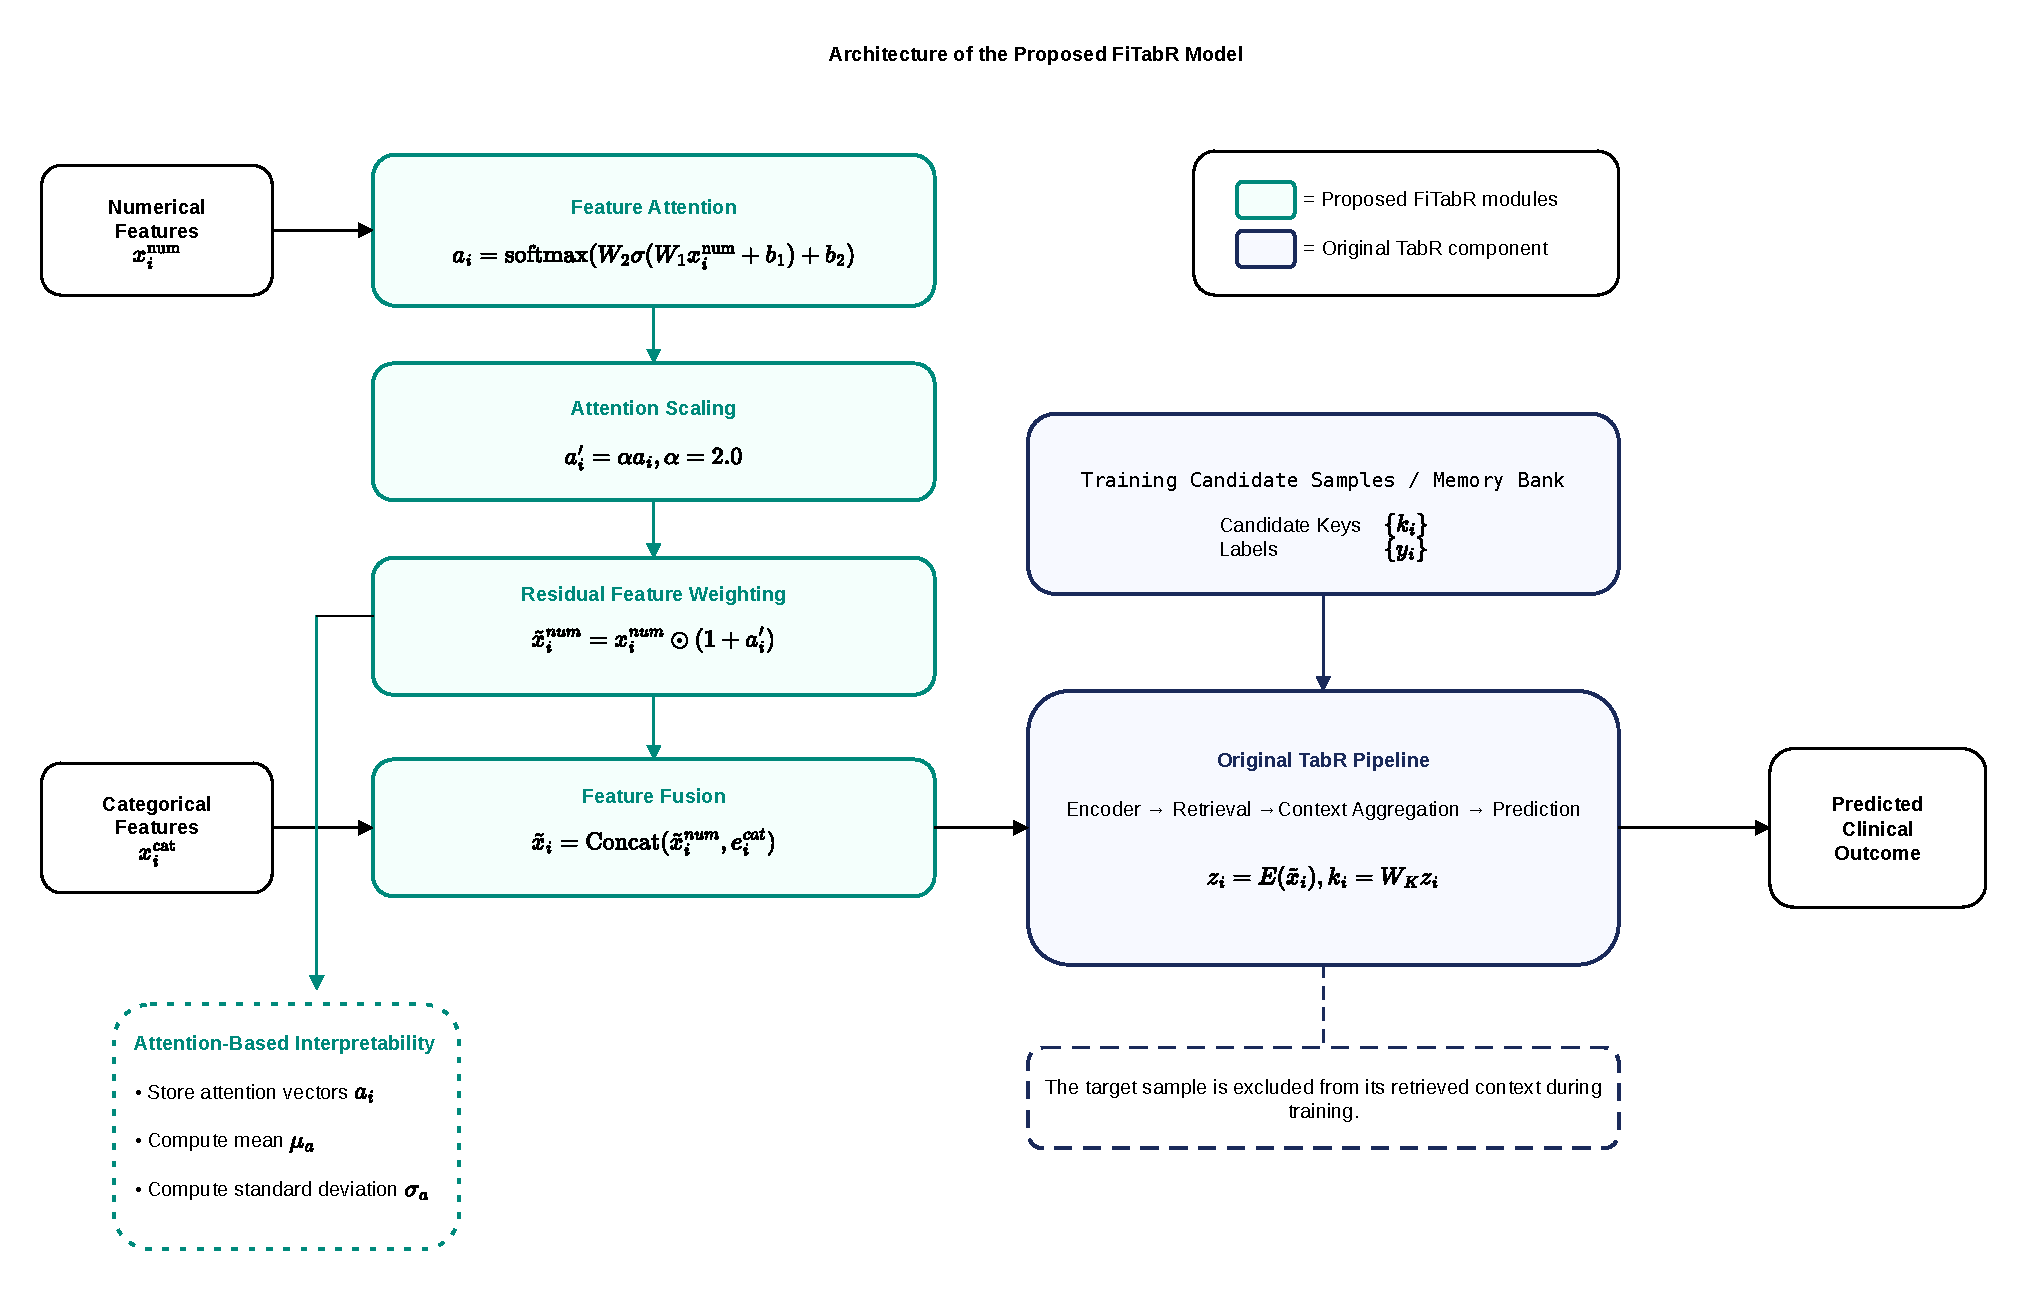
\includegraphics[width=\textwidth]{graph.drawio.pdf}
\caption{Architecture of the proposed FiTabR model. FiTabR applies feature attention, attention scaling, and residual feature weighting to numerical features before feature fusion and the original TabR retrieval and prediction pipeline.}
\label{fig:fitabr_architecture}
\end{figure}
\section{Base Retrieval Model}

This study uses TabR as the base retrieval-augmented tabular learning architecture. TabR combines neural representation learning with a retrieval mechanism that uses similar training samples as contextual information during prediction. In the proposed FiTabR model, the original TabR retrieval architecture is preserved. The main modification is introduced before the TabR encoder, where numerical features are adaptively reweighted using a feature-attention module. Therefore, this section focuses on the proposed feature-aware representation mechanism rather than re-describing the full TabR architecture.

\section{Proposed FiTabR Architecture}

FiTabR extends TabR by introducing a feature-attention module before the TabR encoder. The motivation for this modification is that not all numerical medical features contribute equally to prediction or patient similarity. In clinical datasets, some variables may be highly informative for a specific disease prediction task, while others may be weakly related or noisy. Therefore, treating all numerical features uniformly before retrieval may reduce the quality of the retrieved neighborhood.

The proposed FiTabR pipeline follows the sequence 
$x_i^{\mathrm{num}} \rightarrow a_i \rightarrow \tilde{x}_i^{\mathrm{num}} \rightarrow \tilde{x}_i \rightarrow z_i \rightarrow k_i \rightarrow \hat{y}_i$. First, the numerical input is passed through a feature-attention module to obtain the attention vector $a_i$. The attention vector is then used to generate the weighted numerical representation $\tilde{x}_i^{\mathrm{num}}$. After feature fusion, the final feature-aware representation $\tilde{x}_i$ is passed into the TabR architecture for retrieval-based prediction.

This design keeps the main TabR retrieval structure unchanged while adding a feature-aware preprocessing stage before representation learning and retrieval.The proposed modification is motivated by the assumption that retrieval quality in TabR depends strongly on the representation used to compute candidate similarity. In medical tabular datasets, numerical variables often differ in diagnostic relevance, measurement scale, and noise level. If all numerical features are encoded uniformly, weak or noisy features may affect the learned representation and consequently degrade neighborhood retrieval. Therefore, FiTabR introduces a feature-attention module before the TabR encoder to adaptively emphasize informative numerical variables while preserving the original retrieval mechanism.

\section{Feature-Attention Module}

The feature-attention module is applied to the numerical feature vector $x_i^{\mathrm{num}}$. The attention vector $a_i$ is computed as

\begin{equation}
a_i =
\operatorname{softmax}
\left(
W_2 \sigma \left(W_1 x_i^{\mathrm{num}} + b_1\right) + b_2
\right),
\label{eq:feature_attention}
\end{equation}

where $W_1$ and $W_2$ are trainable weight matrices, $b_1$ and $b_2$ are bias terms, and $\sigma(\cdot)$ denotes the ReLU activation function. The softmax function normalizes the attention scores across numerical features, allowing the model to assign sample-specific importance to each numerical variable.

The trainable matrices $W_1$ and $W_2$, together with the bias terms $b_1$ and $b_2$, allow the model to learn nonlinear relationships between numerical features and their importance. Therefore, the feature-attention module can adaptively emphasize features that are more relevant for constructing the retrieval representation.

\section{Attention Scaling and Residual Feature Weighting}

After computing the attention vector $a_i$, FiTabR scales it using $a_i' = \alpha a_i$, where $\alpha$ is the attention scaling coefficient. In the current implementation, $\alpha = 2.0$. This scaling step increases the influence of the attention vector before it is applied to the original numerical input. Direct attention weighting may suppress original clinical measurements too aggressively, especially in small medical datasets. The residual form preserves the original feature values and only amplifies features selected by the learned attention vector. The value α=2.0 is used as an implementation-level scaling coefficient and is examined empirically in the experimental analysis.

The scaled attention vector $a_i'$ is then applied to the original numerical input through residual feature weighting:

\begin{equation}
\tilde{x}_i^{\mathrm{num}}
=
x_i^{\mathrm{num}}
\odot
\left(1 + a_i'\right),
\label{eq:residual_feature_weighting}
\end{equation}

where $\odot$ denotes element-wise multiplication. The residual term $1 + a_i'$ preserves the original numerical feature values while allowing the model to amplify selected features. Thus, the attention mechanism acts as a learned feature enhancement step rather than replacing the original input.

\section{Feature Fusion}

After residual feature weighting, the weighted numerical representation $\tilde{x}_i^{\mathrm{num}}$ is combined with the encoded categorical representation $e_i^{\mathrm{cat}}$. The fused feature-aware representation is defined as 
$\tilde{x}_i = \operatorname{Concat}(\tilde{x}_i^{\mathrm{num}}, e_i^{\mathrm{cat}})$. This representation is then passed to the TabR encoder.

The role of this step is to ensure that both numerical and categorical information are available to the TabR encoder. FiTabR modifies the numerical feature representation through attention, while categorical features are preserved through their encoded representation.

\section{Integration with TabR Retrieval}

After feature weighting and feature fusion, the resulting representation $\tilde{x}_i$ is passed into the original TabR architecture. The TabR encoder produces the latent representation $z_i = E(\tilde{x}_i)$, which is projected into the retrieval key space as $k_i = W_K z_i$, where $W_K$ is a learnable key projection matrix.

For a target sample $q$, the similarity between the target representation and a candidate sample $i$ is computed using the negative squared Euclidean distance:

\begin{equation}
S(z_q, z_i)
=
-
\left\|k_q - k_i\right\|_2^2.
\label{eq:retrieval_similarity}
\end{equation}

Candidate samples with higher similarity scores are retrieved as contextual samples. FiTabR does not modify the similarity function, neighbor retrieval mechanism, contextual value construction, or prediction head of TabR. Instead, it changes the representation that enters the retrieval pipeline by applying feature-aware numerical weighting before encoding.

For each retrieved candidate sample, the contextual value representation is computed as

\begin{equation}
V(z_q, z_i, y_i)
=
W_Y(y_i) + T(k_q - k_i),
\label{eq:contextual_value}
\end{equation}

where $W_Y(y_i)$ denotes the label embedding of the retrieved candidate sample and $T(\cdot)$ is a learnable transformation of the difference between the target key and the candidate key. The retrieved contextual values are aggregated into $C_q$, and the prediction head produces the final output $\hat{y}_q = P(z_q, C_q)$.

This design isolates the contribution of FiTabR to the feature-representation stage. As a result, any performance difference between TabR and FiTabR can be interpreted as the effect of adding feature-aware numerical weighting before retrieval.

\section{Attention-Based Interpretability}

FiTabR stores the attention vectors produced by the feature-attention module. Since each attention vector $a_i$ is computed for an individual sample, these values can be analyzed to understand which numerical features receive higher emphasis before retrieval.

To summarize feature-attention behavior across the dataset, FiTabR computes the mean attention score 
$\mu_a = \frac{1}{N}\sum_{i=1}^{N} a_i$. It also computes the standard deviation 
$\sigma_a = \sqrt{\frac{1}{N}\sum_{i=1}^{N}(a_i - \mu_a)^2}$. The mean attention score indicates the average attention assigned to each numerical feature, while the standard deviation shows how much attention varies across samples.

These attention statistics provide an additional interpretability signal. However, they should not be interpreted as complete clinical explanations. Instead, they indicate which numerical features the model emphasizes before retrieval and should be analyzed together with predictive performance, retrieved-neighbor behavior, and medical domain knowledge.

\section{Methodological Summary}

FiTabR preserves the retrieval-based structure of TabR while introducing a feature-attention module before the retrieval stage. The proposed method first computes sample-specific attention scores for numerical features, then applies residual feature weighting to construct a feature-aware numerical representation. The weighted representation is then passed into the TabR retrieval architecture, where similar samples are retrieved and used as contextual information for prediction.

This design allows FiTabR to preserve the original retrieval-augmented learning behavior of TabR while introducing a lightweight mechanism for feature-aware representation construction. As a result, the model can emphasize informative numerical variables before retrieval and provide attention statistics that support interpretation.

    
\chapter{Experimental Setup}
\addcontentsline{toc}{chapter}{Experimental Setup}
\label{chap:experimental-setup}
FiTabR was evaluated on three medical tabular binary-classification datasets. The experimental protocol covered data partitioning, preprocessing, baseline selection, hyperparameter optimisation, repeated training, and final test-set evaluation. All models were evaluated using the same data partitions and metric implementations. For the direct architectural comparison, FiTabR and the reference retrieval-based model additionally used the same candidate memory, retrieval configuration, optimisation objective, and random seeds. The implementation was developed using the experimental framework of the reference architecture~\cite{gorishniy2024tabr}.

\section{Datasets}
\label{sec:datasets}

Experiments were conducted on the Heart Disease, Pima Indians Diabetes, and Stroke Prediction datasets~\cite{heartdataset,pimadataset,strokedataset}. The datasets represent different clinical prediction tasks and vary in sample size, feature composition, and class distribution. All tasks were formulated as supervised binary classification. For an observation $x_i$, the corresponding target was denoted by $y_i\in\{0,1\}$.

\subsection{Heart Disease}

The Heart Disease dataset contains 918 observations, six numerical features, and five categorical features. The objective is to predict the presence or absence of heart disease from demographic characteristics, symptoms, and clinical measurements. The processed data were divided into 642 training samples, 138 validation samples, and 138 test samples.

\subsection{Pima Indians Diabetes}

The Pima Indians Diabetes dataset contains 768 observations and eight numerical features. The prediction target indicates whether a patient has diabetes based on diagnostic measurements, including glucose concentration, blood pressure, body mass index, insulin level, age, and pregnancy history. The processed data were divided into 537 training samples, 115 validation samples, and 116 test samples.

\subsection{Stroke Prediction}

The Stroke Prediction dataset contains 5,110 observations, five numerical features, and five categorical features. The objective is to predict stroke occurrence from demographic information, medical history, lifestyle indicators, and physiological measurements. The processed data were divided into 3,577 training samples, 766 validation samples, and 767 test samples. Because the positive class is substantially less frequent than the negative class, threshold-independent and class-sensitive metrics were included in the evaluation.

\begin{table}[t]
\caption{Summary of the Medical Tabular Datasets}
\label{tab:datasets}
\centering
\small
\begin{tabular}{lrrrr}
\toprule
Dataset & Samples & Numerical & Categorical & Task \\
\midrule
Heart Disease & 918 & 6 & 5 & Binary \\
Pima Diabetes & 768 & 8 & 0 & Binary \\
Stroke Prediction & 5,110 & 5 & 5 & Binary \\
\bottomrule
\end{tabular}
\end{table}

The selected datasets reflect common constraints in medical tabular learning, including limited sample size, heterogeneous variables, unequal feature scales, missing observations, and class imbalance. Evaluating the same architecture across the three datasets therefore provides evidence regarding the consistency of the proposed feature-aware representation mechanism under different clinical data conditions.

\section{Preprocessing}
\label{sec:preprocessing}

A common preprocessing pipeline was applied to all models. Each preprocessing operation was fitted using only the training partition and was subsequently applied to the validation and test partitions without refitting. This procedure prevented validation or test information from influencing model training.

Each dataset was divided into disjoint training, validation, and test subsets using an approximate ratio of 70:15:15. Stratified partitioning was used to preserve the class distribution across the subsets. The training subset was used to estimate model parameters, the validation subset was used for hyperparameter selection and early stopping, and the test subset was reserved for final evaluation.

Numerical features were processed using quantile transformation. This operation reduced the effect of extreme values and differences in feature scale. The transformation was estimated from the training subset and then applied to the validation and test subsets. Categorical variables were integer encoded using mappings derived from the training data. The same mappings were retained for the remaining subsets.

Missing numerical values were imputed using statistics calculated from the training subset. Missing categorical values were represented by a dedicated category or processed according to the categorical policy supported by the corresponding model. Validation- and test-set statistics were not used during imputation.

Synthetic oversampling was not applied in the principal experiments. The original class distributions were preserved to avoid introducing artificial observations into the retrieval candidate memory. The effects of class imbalance were assessed using recall, F1-score, and receiver operating characteristic area under the curve (ROC--AUC), in addition to accuracy.

For the retrieval-based models, the candidate memory contained only training observations. Validation and test observations were not inserted into the memory. During training, the current target observation was excluded from its own candidate context. These restrictions prevented self-retrieval and label leakage.

\section{Baselines}
\label{sec:baselines}

FiTabR was compared with gradient-boosted decision trees, conventional neural networks, attention-based deep tabular models, and the original retrieval-based architecture. The selected baselines cover the principal model families commonly used for supervised tabular classification.

\subsection{Gradient-Boosted Decision Trees}

XGBoost~\cite{chen2016xgboost}, LightGBM~\cite{ke2017lightgbm}, and CatBoost~\cite{prokhorenkova2018catboost} were used as tree-based baselines. These methods provide strong non-deep-learning reference points for small and medium-sized tabular datasets. CatBoost was also included because the Heart Disease and Stroke Prediction datasets contain categorical variables.

\subsection{Deep Tabular Models}

A multilayer perceptron (MLP) was used as the basic neural-network baseline.\cite{gorishniy2021revisiting} The MLP processes each observation independently and does not use feature attention or retrieved training instances. FT-Transformer~\cite{fttransformer} represents individual features as tokens and applies self-attention to model interactions among features. SAINT~\cite{somepalli2021saint} provides an additional attention-based comparison for tabular representation learning.

\subsection{Retrieval-Based Baseline}

The original retrieval-based architecture TabR~\cite{gorishniy2024tabr} was used as the principal architectural baseline. FiTabR preserves its candidate retrieval, context aggregation, and prediction framework while modifying the input representation through feature attention, residual feature weighting, and feature fusion. This design supports a controlled assessment of whether the proposed representation module improves similarity learning and downstream classification.

\section{Evaluation Metrics}
\label{sec:metrics}

Performance was evaluated using accuracy, precision, recall, F1-score, ROC--AUC, and binary cross-entropy. The first four metrics were computed from the classification decisions, whereas ROC--AUC and binary cross-entropy were computed from predicted probabilities.

\subsection{Accuracy}

Accuracy measures the proportion of correctly classified observations:
\begin{equation}
\mathrm{Accuracy}=
\frac{TP+TN}{TP+TN+FP+FN},
\label{eq:accuracy}
\end{equation}
where $TP$, $TN$, $FP$, and $FN$ denote true positives, true negatives, false positives, and false negatives, respectively.

\subsection{Precision and Recall}

Precision measures the proportion of positive predictions that are correct:
\begin{equation}
\mathrm{Precision}=\frac{TP}{TP+FP}.
\label{eq:precision}
\end{equation}
Recall measures the proportion of positive observations correctly identified:
\begin{equation}
\mathrm{Recall}=\frac{TP}{TP+FN}.
\label{eq:recall}
\end{equation}
Recall is particularly relevant to medical classification because false-negative predictions may cause affected patients to be missed.

\subsection{F1-Score}

The F1-score is the harmonic mean of precision and recall:
\begin{equation}
\mathrm{F1}=2\frac{\mathrm{Precision}\times\mathrm{Recall}}
{\mathrm{Precision}+\mathrm{Recall}}.
\label{eq:f1}
\end{equation}
It provides a balanced measure when both false-positive and false-negative errors are relevant.

\subsection{ROC--AUC}

ROC--AUC measures the ability of a model to rank positive observations above negative observations across classification thresholds. A value of 0.5 indicates random ranking, whereas a value of 1.0 indicates perfect class discrimination. This metric was included because it is less dependent on a single decision threshold than accuracy or F1-score.

\subsection{Binary Cross-Entropy}

Binary cross-entropy evaluates the quality of the predicted probabilities:
\begin{equation}
\mathcal{L}_{\mathrm{BCE}}=-\frac{1}{N}\sum_{i=1}^{N}
\left[y_i\log(\hat{p}_i)+(1-y_i)\log(1-\hat{p}_i)\right],
\label{eq:bce}
\end{equation}
where $y_i$ is the true label and $\hat{p}_i$ is the predicted probability of the positive class. Lower values indicate better probabilistic predictions.

For the imbalanced Stroke Prediction dataset, ROC--AUC, recall, and F1-score were considered together with accuracy. This avoided drawing conclusions from majority-class performance alone.

\section{Implementation Details}
\label{sec:implementation-details}

The models were implemented in Python using a shared experimental framework. Dataset processing and metric computation were based on scikit-learn~\cite{sklearn}. Hyperparameter optimisation was performed using Optuna with the Tree-structured Parzen Estimator sampler~\cite{optuna}. The repository configurations used 200 optimisation trials, including 20 initial startup trials. Hyperparameter selection was based exclusively on validation performance.

For neural models, the search space included learning rate, weight decay, hidden representation dimension, number of processing blocks, batch size, and dropout. Attention-based models additionally included attention dropout and attention-specific representation parameters. For FiTabR, parameters associated with feature attention, residual scaling, and feature fusion were included in the optimisation procedure.

For the tree-based baselines, the search space included learning rate, tree depth, number of boosting iterations, regularisation coefficients, bagging parameters, and leaf-estimation settings. Early stopping was applied using the validation subset.

Neural models were trained by mini-batch gradient-based optimisation using binary cross-entropy as the objective function. The candidate memory for retrieval-based training consisted of the complete training partition. The retrieval configuration was kept fixed between FiTabR and the architectural baseline so that the primary experimental difference was the proposed feature-aware input representation.

Each selected configuration was evaluated using 15 random seeds, numbered from 0 to 14. The trained models were divided into three groups:
\begin{equation}
\{0,1,2,3,4\},\quad
\{5,6,7,8,9\},\quad
\{10,11,12,13,14\}.
\label{eq:seed-groups}
\end{equation}
Predicted probabilities were averaged within each group to form three five-model ensembles. For a metric $m$, the mean over $R$ runs was calculated as
\begin{equation}
\bar{m}=\frac{1}{R}\sum_{r=1}^{R}m_r,
\label{eq:metric-mean}
\end{equation}
and the standard deviation was calculated as
\begin{equation}
s_m=\sqrt{\frac{1}{R-1}\sum_{r=1}^{R}(m_r-\bar{m})^2}.
\label{eq:metric-std}
\end{equation}

The direct comparison between FiTabR and the architectural baseline used identical preprocessing, data partitions, candidate memory, retrieval settings, optimisation objective, early-stopping procedure, random seeds, and evaluation metrics. The principal difference was the feature-aware representation module introduced before the encoder.

% Replace the bracketed fields below after verifying the final environment.
All experiments were conducted using Python 3.9.16 and PyTorch 1.13.1
on a system equipped with an Intel Core i7-7700K CPU operating at
4.20 GHz, 32 GB of RAM, and an NVIDIA GeForce GTX 1050 GPU with
2 GB of dedicated memory. The software environment included CUDA
11.7.99, scikit-learn 1.2.2, XGBoost 1.7.4, LightGBM 3.3.5,
CatBoost 1.1.1, and Optuna 3.1.0.

\chapter{Results and Discussion}
\label{chap:results}

This section evaluates the predictive performance of FiTabR against the
original TabR architecture and representative machine-learning and
deep-learning baselines on the Heart Disease, Pima Diabetes, and Stroke
Prediction datasets. The baselines include the gradient-boosted tree methods CatBoost, XGBoost,
and LightGBM \cite{prokhorenkova2018catboost,chen2016xgboost,ke2017lightgbm},
together with an MLP and the tabular deep-learning models SAINT and
FT-Transformer \cite{somepalli2021saint,gorishniy2021revisiting}. TabR is
included as the direct retrieval-augmented architectural baseline
\cite{gorishniy2024tabr}. The reported values correspond to ensemble
evaluation and are expressed as mean $\pm$ standard deviation. Precision,
recall, and F1-score in the aggregate comparison are weighted averages unless
otherwise stated. Accuracy, precision, recall, F1-score, and ROC-AUC are
maximized, whereas lower cross-entropy indicates better probabilistic
prediction.



\section{Overall Comparison With All Baselines}

Tables~\ref{tab:heart_results}--\ref{tab:stroke_results} summarize the
performance of the evaluated models. The results show that no single model
dominates across all datasets and evaluation criteria. The relative
performance of tree-based and deep-learning methods varies across datasets,
while FiTabR is most competitive on the Heart Disease dataset.

\begin{table}[H]
\centering
\caption{Performance comparison on the Heart Disease dataset. Results are
reported as mean $\pm$ standard deviation. \\}
\label{tab:heart_results}
\resizebox{\textwidth}{!}{
\begin{tabular}{lcccccc}
\hline
\textbf{Model} &
\textbf{Accuracy} &
\textbf{Precision} &
\textbf{Recall} &
\textbf{F1-score} &
\textbf{ROC-AUC} &
\textbf{Cross-Entropy} \\
\hline
CatBoost &
$0.8889 \pm 0.0042$ &
$0.8896 \pm 0.0043$ &
$0.8889 \pm 0.0042$ &
$0.8890 \pm 0.0042$ &
$0.9334 \pm 0.0001$ &
$0.3390 \pm 0.0060$ \\

XGBoost &
$0.8841 \pm 0.0000$ &
$0.8856 \pm 0.0008$ &
$0.8841 \pm 0.0000$ &
$0.8843 \pm 0.0001$ &
$0.9341 \pm 0.0030$ &
$0.3481 \pm 0.0146$ \\

LightGBM &
$0.8841 \pm 0.0000$ &
$0.8847 \pm 0.0000$ &
$0.8841 \pm 0.0000$ &
$0.8842 \pm 0.0000$ &
$0.9428 \pm 0.0005$ &
$0.3281 \pm 0.0086$ \\

MLP &
$0.8720 \pm 0.0042$ &
$0.8729 \pm 0.0045$ &
$0.8720 \pm 0.0042$ &
$0.8722 \pm 0.0042$ &
$0.9351 \pm 0.0007$ &
$0.3350 \pm 0.0031$ \\

SAINT &
$0.8792 \pm 0.0221$ &
$0.8814 \pm 0.0205$ &
$0.8792 \pm 0.0221$ &
$0.8795 \pm 0.0220$ &
$0.9390 \pm 0.0011$ &
$0.3322 \pm 0.0186$ \\

FT-Transformer &
$0.8696 \pm 0.0072$ &
$0.8716 \pm 0.0064$ &
$0.8696 \pm 0.0072$ &
$0.8698 \pm 0.0072$ &
$0.9344 \pm 0.0037$ &
$0.3582 \pm 0.0098$ \\

TabR &
$0.8841 \pm 0.0000$ &
$0.8880 \pm 0.0000$ &
$0.8841 \pm 0.0000$ &
$0.8844 \pm 0.0000$ &
$\mathbf{0.9510 \pm 0.0006}$ &
$0.3586 \pm 0.0267$ \\

\textbf{FiTabR} &
$\mathbf{0.8937 \pm 0.0042}$ &
$\mathbf{0.8977 \pm 0.0043}$ &
$\mathbf{0.8937 \pm 0.0042}$ &
$\mathbf{0.8940 \pm 0.0042}$ &
$\mathbf{0.9510 \pm 0.0009}$ &
$\mathbf{0.3038 \pm 0.0097}$ \\
\hline
\end{tabular}}
\end{table}

On Heart Disease, FiTabR achieves the strongest overall results among the
evaluated models. In particular, it obtains the highest mean accuracy,
precision, recall, and F1-score, while its ROC-AUC is effectively tied with
TabR at approximately 0.951. FiTabR also records the lowest cross-entropy,
suggesting improved confidence and probabilistic prediction. CatBoost is the
closest conventional baseline in terms of accuracy, whereas LightGBM obtains
the strongest ROC-AUC among the non-retrieval models. The result therefore
indicates that the proposed feature-aware representation is particularly
effective on this dataset.

\begin{table}[H]
\centering
\caption{Performance comparison on the Pima Diabetes dataset. Results are
reported as mean $\pm$ standard deviation.\\}
\label{tab:pima_results}
\resizebox{\textwidth}{!}{
\begin{tabular}{lcccccc}
\hline
\textbf{Model} &
\textbf{Accuracy} &
\textbf{Precision} &
\textbf{Recall} &
\textbf{F1-score} &
\textbf{ROC-AUC} &
\textbf{Cross-Entropy} \\
\hline
CatBoost &
$0.7586 \pm 0.0086$ &
$0.7550 \pm 0.0083$ &
$0.7586 \pm 0.0086$ &
$0.7554 \pm 0.0080$ &
$0.7918 \pm 0.0035$ &
$0.6831 \pm 0.0029$ \\

XGBoost &
$0.7672 \pm 0.0000$ &
$0.7636 \pm 0.0002$ &
$0.7672 \pm 0.0000$ &
$0.7610 \pm 0.0011$ &
$0.8078 \pm 0.0034$ &
$0.5895 \pm 0.0236$ \\

LightGBM &
$0.7500 \pm 0.0149$ &
$0.7467 \pm 0.0159$ &
$0.7500 \pm 0.0149$ &
$0.7437 \pm 0.0132$ &
$0.8086 \pm 0.0060$ &
$\mathbf{0.5253 \pm 0.0023}$ \\

MLP &
$0.7644 \pm 0.0050$ &
$0.7633 \pm 0.0071$ &
$0.7644 \pm 0.0050$ &
$0.7635 \pm 0.0065$ &
$0.7918 \pm 0.0054$ &
$0.5659 \pm 0.0185$ \\

SAINT &
$0.7529 \pm 0.0100$ &
$0.7638 \pm 0.0073$ &
$0.7529 \pm 0.0100$ &
$0.7558 \pm 0.0095$ &
$0.8054 \pm 0.0003$ &
$0.5339 \pm 0.0048$ \\

FT-Transformer &
$\mathbf{0.7701 \pm 0.0263}$ &
$\mathbf{0.7774 \pm 0.0203}$ &
$\mathbf{0.7701 \pm 0.0263}$ &
$\mathbf{0.7722 \pm 0.0250}$ &
$\mathbf{0.8135 \pm 0.0071}$ &
$0.5337 \pm 0.0223$ \\

TabR &
$0.7529 \pm 0.0050$ &
$0.7515 \pm 0.0062$ &
$0.7529 \pm 0.0050$ &
$0.7520 \pm 0.0058$ &
$0.7963 \pm 0.0072$ &
$0.5511 \pm 0.0120$ \\

\textbf{FiTabR} &
$0.7586 \pm 0.0086$ &
$0.7595 \pm 0.0099$ &
$0.7586 \pm 0.0086$ &
$0.7589 \pm 0.0092$ &
$0.7953 \pm 0.0047$ &
$0.5474 \pm 0.0044$ \\
\hline
\end{tabular}}
\end{table}

The Pima Diabetes dataset produces a more competitive ordering among the
model families. FT-Transformer achieves the highest mean accuracy,
precision, recall, F1-score, and ROC-AUC, while LightGBM obtains the lowest
cross-entropy. FiTabR therefore does not provide the best absolute
performance on this dataset. Nevertheless, its comparison with TabR remains
important because the two architectures differ primarily in the proposed
feature-aware input representation. FiTabR improves the main
threshold-dependent classification metrics and reduces cross-entropy, while
its ROC-AUC remains close to that of TabR.

\begin{table}[t]
\centering
\caption{Performance comparison on the Stroke Prediction dataset. Results
are reported as mean $\pm$ standard deviation.\\}
\label{tab:stroke_results}
\resizebox{\textwidth}{!}{
\begin{tabular}{lcccccc}
\hline
\textbf{Model} &
\textbf{Accuracy} &
\textbf{Precision} &
\textbf{Recall} &
\textbf{F1-score} &
\textbf{ROC-AUC} &
\textbf{Cross-Entropy} \\
\hline
CatBoost &
$0.9500 \pm 0.0008$ &
$0.9033 \pm 0.0000$ &
$0.9500 \pm 0.0008$ &
$0.9261 \pm 0.0004$ &
$0.8294 \pm 0.0168$ &
$0.3105 \pm 0.0525$ \\

XGBoost &
$0.9513 \pm 0.0008$ &
$\mathbf{0.9407 \pm 0.0125}$ &
$0.9513 \pm 0.0008$ &
$\mathbf{0.9300 \pm 0.0016}$ &
$0.8201 \pm 0.0024$ &
$0.2259 \pm 0.0678$ \\

LightGBM &
$\mathbf{0.9518 \pm 0.0013}$ &
$0.9376 \pm 0.0296$ &
$\mathbf{0.9518 \pm 0.0013}$ &
$0.9294 \pm 0.0031$ &
$0.8199 \pm 0.0023$ &
$\mathbf{0.1640 \pm 0.0007}$ \\

MLP &
$0.9505 \pm 0.0000$ &
$0.9034 \pm 0.0000$ &
$0.9505 \pm 0.0000$ &
$0.9263 \pm 0.0000$ &
$0.8220 \pm 0.0087$ &
$0.1738 \pm 0.0129$ \\

SAINT &
$0.9505 \pm 0.0000$ &
$0.9034 \pm 0.0000$ &
$0.9505 \pm 0.0000$ &
$0.9263 \pm 0.0000$ &
$0.7368 \pm 0.0528$ &
$0.2042 \pm 0.0067$ \\

FT-Transformer &
$0.9505 \pm 0.0000$ &
$0.9034 \pm 0.0000$ &
$0.9505 \pm 0.0000$ &
$0.9263 \pm 0.0000$ &
$\mathbf{0.8328 \pm 0.0036}$ &
$0.1663 \pm 0.0049$ \\

TabR &
$0.9505 \pm 0.0000$ &
$0.9034 \pm 0.0000$ &
$0.9505 \pm 0.0000$ &
$0.9263 \pm 0.0000$ &
$0.8136 \pm 0.0078$ &
$0.1780 \pm 0.0050$ \\

\textbf{FiTabR} &
$0.9505 \pm 0.0000$ &
$0.9034 \pm 0.0000$ &
$0.9505 \pm 0.0000$ &
$0.9263 \pm 0.0000$ &
$0.8095 \pm 0.0126$ &
$0.1750 \pm 0.0091$ \\
\hline
\end{tabular}}
\end{table}

On Stroke Prediction, the aggregate accuracy of almost all models is close
to 0.95. LightGBM achieves the highest mean accuracy and recall, XGBoost
obtains the highest precision and F1-score, and FT-Transformer provides the
highest ROC-AUC. FiTabR and TabR obtain identical accuracy, precision,
recall, and F1-score, while FiTabR slightly reduces cross-entropy from
$0.1780$ to $0.1750$. In contrast, the mean ROC-AUC decreases from
$0.8136$ for TabR to $0.8095$ for FiTabR. The high aggregate accuracy,
however, requires further analysis because the Stroke dataset is strongly
imbalanced.

\subsection{Direct TabR--FiTabR Comparison}

Since FiTabR is constructed as an extension of TabR, the direct comparison
between these two models provides the most controlled evaluation of the
proposed feature-aware representation. The retrieval, aggregation, and
prediction framework is retained, while FiTabR introduces feature-dependent
representation learning before the TabR encoder.

On Heart Disease, FiTabR improves accuracy from
$0.8841 \pm 0.0000$ to $0.8937 \pm 0.0042$, corresponding to an absolute
increase of approximately 0.96 percentage points. Precision increases from
0.8880 to 0.8977, recall from 0.8841 to 0.8937, and F1-score from 0.8844 to
0.8940. The two models obtain essentially identical mean ROC-AUC
($0.9510$), whereas FiTabR reduces cross-entropy from
$0.3586 \pm 0.0267$ to $0.3038 \pm 0.0097$. Thus, the principal improvement
on Heart Disease occurs in final classification behavior and probabilistic
prediction rather than in ranking performance.

On Pima Diabetes, FiTabR improves accuracy from
$0.7529 \pm 0.0050$ to $0.7586 \pm 0.0086$ and F1-score from
$0.7520 \pm 0.0058$ to $0.7589 \pm 0.0092$. Precision and recall exhibit the
same direction of change, and cross-entropy decreases from 0.5511 to 0.5474.
The ROC-AUC difference is small and favors TabR, with mean values of 0.7963
and 0.7953, respectively. Therefore, the feature-aware representation
provides modest gains in threshold-dependent metrics but does not improve
ranking performance on Pima Diabetes.

On Stroke Prediction, the two retrieval models obtain identical mean
accuracy, precision, recall, and F1-score. FiTabR produces a small reduction
in cross-entropy but a lower mean ROC-AUC. The direct comparison therefore
shows that the benefit of feature-aware representation is dataset-dependent,
with the clearest improvement occurring on Heart Disease.

\subsection{Heart Disease Results}

The Heart Disease dataset provides the strongest quantitative support for
FiTabR. The proposed model achieves an accuracy of
$0.8937 \pm 0.0042$, exceeding TabR, CatBoost, XGBoost, LightGBM, MLP,
SAINT, and FT-Transformer. The same ordering is observed for precision,
recall, and F1-score. In particular, FiTabR obtains an F1-score of
$0.8940 \pm 0.0042$, compared with $0.8890 \pm 0.0042$ for CatBoost and
$0.8844 \pm 0.0000$ for TabR.

The ROC-AUC comparison is more conservative. FiTabR and TabR both obtain a
mean value of approximately 0.9510, considerably above the remaining
baselines, but the difference between the two retrieval models is
negligible. Accordingly, the results do not support a claim that FiTabR
improves the ranking capability of TabR on Heart Disease.

A clearer distinction appears in cross-entropy. FiTabR obtains
$0.3038 \pm 0.0097$, compared with $0.3586 \pm 0.0267$ for TabR and
$0.3281 \pm 0.0086$ for LightGBM. This is the lowest mean cross-entropy in
the comparison. Taken together, the Heart Disease results indicate that
feature-aware representation improves the classification output and
probabilistic quality of the retrieval-based model while preserving the
strong ROC-AUC performance of TabR.

\subsection{Pima Diabetes Results}

Performance on Pima Diabetes is less concentrated around a single model.
FT-Transformer obtains the highest mean accuracy
($0.7701 \pm 0.0263$), precision ($0.7774 \pm 0.0203$), recall
($0.7701 \pm 0.0263$), F1-score ($0.7722 \pm 0.0250$), and ROC-AUC
($0.8135 \pm 0.0071$). LightGBM achieves the lowest cross-entropy at
$0.5253 \pm 0.0023$.

FiTabR is therefore not the strongest model in absolute terms on this
dataset. Nevertheless, it improves its direct TabR baseline on four
classification metrics. Accuracy increases from $0.7529$ to $0.7586$,
precision from $0.7515$ to $0.7595$, recall from $0.7529$ to $0.7586$, and
F1-score from $0.7520$ to $0.7589$. Cross-entropy is also reduced from
0.5511 to 0.5474.

The mean ROC-AUC changes from $0.7963 \pm 0.0072$ for TabR to
$0.7953 \pm 0.0047$ for FiTabR. Given both the small magnitude of the
difference and the reported variability, the results should be interpreted
as showing no meaningful improvement in ranking performance. Thus, on Pima
Diabetes, FiTabR provides a modest improvement in threshold-based
classification behavior but remains behind the strongest alternative
baselines.

\subsection{Stroke Prediction and Minority-Class Behavior}

The Stroke Prediction dataset presents a substantially different evaluation
scenario because of its severe class imbalance. Although the aggregate
accuracy is approximately 0.95 for TabR and FiTabR, this value alone does
not describe the ability of the models to detect Stroke cases.

To examine this issue directly, Table~\ref{tab:stroke_minority} reports
positive-class and class-balanced metrics for the two retrieval models.

\begin{table}[t]
\centering
\caption{Minority-class performance of TabR and FiTabR on the Stroke
Prediction dataset.\\}
\label{tab:stroke_minority}
\resizebox{\columnwidth}{!}{
\begin{tabular}{lcccccc}
\hline
\textbf{Model} &
\textbf{Pos. Prec.} &
\textbf{Pos. Rec.} &
\textbf{Pos. F1} &
\textbf{Macro F1} &
\textbf{Bal. Acc.} &
\textbf{ROC-AUC} \\
\hline
TabR &
$0.0000 \pm 0.0000$ &
$0.0000 \pm 0.0000$ &
$0.0000 \pm 0.0000$ &
$0.4873 \pm 0.0000$ &
$0.5000 \pm 0.0000$ &
$0.8136 \pm 0.0078$ \\

FiTabR &
$0.0000 \pm 0.0000$ &
$0.0000 \pm 0.0000$ &
$0.0000 \pm 0.0000$ &
$0.4873 \pm 0.0000$ &
$0.5000 \pm 0.0000$ &
$0.8095 \pm 0.0126$ \\
\hline
\end{tabular}}
\end{table}

The minority-class results reveal that both TabR and FiTabR fail to predict
positive Stroke cases at the default classification threshold. Positive
precision, recall, and F1-score are all zero, while balanced accuracy is
exactly 0.5000 and macro F1-score is 0.4873. Consequently, the approximately
95\% aggregate accuracy of both models is driven by correct prediction of
the dominant negative class rather than successful discrimination of both
classes.

This distinction is important when interpreting Table~\ref{tab:stroke_results}.
The identical aggregate accuracy and F1-score of TabR and FiTabR should not
be interpreted as evidence of strong clinical classification performance.
FiTabR slightly improves cross-entropy, decreasing it from
$0.1780 \pm 0.0050$ to $0.1750 \pm 0.0091$, but does not resolve the
minority-class detection failure. Its mean ROC-AUC is also slightly lower
than TabR. Therefore, the Stroke experiment identifies a clear limitation of
the current FiTabR formulation: feature-aware representation alone is not
sufficient to overcome severe class imbalance.

\subsection{Cross-Dataset Synthesis}

Across the three medical datasets, the effect of the proposed feature-aware
representation is heterogeneous rather than uniform. Heart Disease provides
the clearest evidence of improvement. FiTabR increases accuracy, precision,
recall, and F1-score relative to TabR, substantially lowers cross-entropy,
and preserves the same strong ROC-AUC. On Pima Diabetes, the improvement is
smaller: FiTabR increases the threshold-dependent classification metrics and
slightly reduces cross-entropy, but does not improve ROC-AUC and remains
behind FT-Transformer and selected GBDT baselines on several metrics.

Stroke Prediction represents the most difficult case. FiTabR does not
improve the aggregate classification metrics over TabR and does not resolve
the failure to identify minority-class examples at the default decision
threshold. The result demonstrates that improvements in feature
representation cannot by themselves compensate for extreme imbalance in
the target distribution.

Overall, the experiments support FiTabR as a targeted extension of TabR
rather than a universally superior replacement. The feature-aware mechanism
provides its strongest benefit on Heart Disease, produces modest gains on
Pima Diabetes, and has limited effect on Stroke Prediction. Importantly, the
comparison with the direct TabR baseline shows that improvements can be
obtained without replacing the underlying retrieval framework. At the same
time, the variation across datasets indicates that the effectiveness of the
proposed representation depends on the characteristics of the underlying
classification problem.

The benchmark results establish the overall predictive behavior of FiTabR,
but they do not identify which elements of the feature-aware representation
are responsible for the observed changes. The following ablation study
therefore isolates residual preservation, fixed attention scaling, and
learned nonuniform weighting. A subsequent feature-attention analysis then
examines the model-internal emphasis assigned to the numerical variables,
without treating the attention values as causal or clinical importance
scores.

\section{Ablation Study}
\label{sec:ablation}

Recall that FiTabR modifies the numerical representation before the
TabR encoder and retrieval stage. As described in the Methodology
section, for the $i$-th sample, the feature-attention module produces
the sample-specific attention vector $a_i$ from the numerical input
$x_i^{\mathrm{num}}$. The attention vector is scaled as

\begin{equation}
a_i' = \alpha a_i,
\qquad \alpha = 2.0,
\label{eq:ablation_scale}
\end{equation}

and the complete FiTabR model applies residual feature weighting as

\begin{equation}
\tilde{x}_i^{\mathrm{num}}
=
x_i^{\mathrm{num}}
\odot
\left(1+a_i'\right),
\label{eq:ablation_fitabr}
\end{equation}

where $\odot$ denotes element-wise multiplication.

To determine which components of this representation mechanism are
important, we evaluate three ablated configurations. The first removes
the residual term, the second removes the fixed attention scaling
coefficient, and the third replaces the learned sample-specific
attention vector with uniform feature weights. TabR is included as the
reference configuration. The resulting numerical representations are

\begin{equation}
\begin{aligned}
\text{TabR:}\quad
&
\tilde{x}_{i}^{\mathrm{num}}
=
x_i^{\mathrm{num}},
\\[3pt]
\text{FiTabR:}\quad
&
\tilde{x}_{i}^{\mathrm{num}}
=
x_i^{\mathrm{num}}
\odot
\left(1+\alpha a_i\right),
\\[3pt]
\text{No Residual:}\quad
&
\tilde{x}_{i,\mathrm{NR}}^{\mathrm{num}}
=
x_i^{\mathrm{num}}
\odot
\left(\alpha a_i\right),
\\[3pt]
\text{No Scale:}\quad
&
\tilde{x}_{i,\mathrm{NS}}^{\mathrm{num}}
=
x_i^{\mathrm{num}}
\odot
\left(1+a_i\right),
\\[3pt]
\text{Uniform:}\quad
&
\tilde{x}_{i,\mathrm{U}}^{\mathrm{num}}
=
x_i^{\mathrm{num}}
\odot
\left(1+\alpha a_i^{\mathrm{U}}\right),
\end{aligned}
\label{eq:ablation_variants}
\end{equation}

where

\begin{equation}
a_i^{\mathrm{U}}
=
\left[
\frac{1}{F},
\ldots,
\frac{1}{F}
\right],
\label{eq:ablation_uniform}
\end{equation}

and $F$ denotes the number of numerical features. All other components
of TabR, including the encoder, candidate retrieval, contextual
aggregation, and prediction head, are kept unchanged. Therefore, the
experiment isolates the effect of the proposed feature-weighting
mechanism.

For each configuration, three independent five-model ensembles are
evaluated, covering 15 trained models in total. The reported values
represent the mean and sample standard deviation across the three
ensembles.


% ============================================================
% Heart Disease
% ============================================================

\subsection{Heart Disease}
\label{subsec:heart_ablation}

Table~\ref{tab:heart_ablation} reports the ablation results on the Heart
Disease dataset. The component columns indicate which elements of the
complete FiTabR representation are retained in each configuration.

\begin{table}[t]
\centering
\caption{Ablation study on the Heart Disease dataset. Results are
reported as mean $\pm$ standard deviation across three five-model
ensembles.\\
}
\label{tab:heart_ablation}

\resizebox{\textwidth}{!}{
\begin{tabular}{lccc|cccc}
\toprule
Model &
Learned $a_i$ &
Residual &
$\alpha=2$ &
Acc. $\uparrow$ &
F1 $\uparrow$ &
AUC $\uparrow$ &
CE $\downarrow$
\\
\midrule

TabR
& $\times$
& $\times$
& $\times$
& 0.8841 $\pm$ 0.0000
& 0.8844 $\pm$ 0.0000
& 0.9510 $\pm$ 0.0006
& 0.3586 $\pm$ 0.0267
\\

FiTabR
& $\checkmark$
& $\checkmark$
& $\checkmark$
& 0.8937 $\pm$ 0.0042
& 0.8940 $\pm$ 0.0042
& 0.9510 $\pm$ 0.0009
& 0.3038 $\pm$ 0.0097
\\

No Residual
& $\checkmark$
& $\times$
& $\checkmark$
& 0.8647 $\pm$ 0.0111
& 0.8651 $\pm$ 0.0110
& 0.9402 $\pm$ 0.0061
& 0.4050 $\pm$ 0.0603
\\

No Scale
& $\checkmark$
& $\checkmark$
& $\times$
& 0.8986 $\pm$ 0.0072
& 0.8988 $\pm$ 0.0072
& 0.9508 $\pm$ 0.0016
& 0.3028 $\pm$ 0.0070
\\

Uniform
& $\times$
& $\checkmark$
& $\checkmark$
& 0.8913 $\pm$ 0.0126
& 0.8916 $\pm$ 0.0125
& 0.9509 $\pm$ 0.0022
& 0.3240 $\pm$ 0.0209
\\

\bottomrule
\end{tabular}
}
\end{table}

The Heart Disease results show the clearest effect of the proposed
representation mechanism. FiTabR improves the mean accuracy from
$0.8841$ for TabR to $0.8937$ and the F1-score from $0.8844$ to
$0.8940$. The ROC-AUC remains essentially unchanged, while
cross-entropy decreases substantially from $0.3586$ to $0.3038$.

Removing the residual term causes the largest deterioration among the
evaluated configurations. Accuracy decreases to $0.8647$, F1-score to
$0.8651$, and ROC-AUC to $0.9402$, while cross-entropy increases to
$0.4050$. This result indicates that retaining the original numerical
representation while applying attention-based modulation is important
for the Heart Disease dataset.

The No Scale configuration obtains the numerically highest accuracy and
F1-score, as well as the lowest mean cross-entropy. However, the
difference between No Scale and complete FiTabR is small relative to the
variation across ensembles. Thus, the experiment does not provide
evidence that the fixed coefficient $\alpha=2.0$ improves performance.
Instead, the learned residual weighting remains effective when the fixed
scaling term is removed.

Uniform weighting is also competitive with the complete model. This
suggests that part of the gain on Heart Disease may originate from
numerical feature modulation itself rather than exclusively from the
learned sample-specific attention distribution. Nevertheless, the
Uniform configuration exhibits greater variability than the complete
FiTabR model.

Figure~\ref{fig:heart_ablation_performance} provides a visual comparison of the
main Heart Disease ablation results.


\begin{figure}[H]
    \centering
    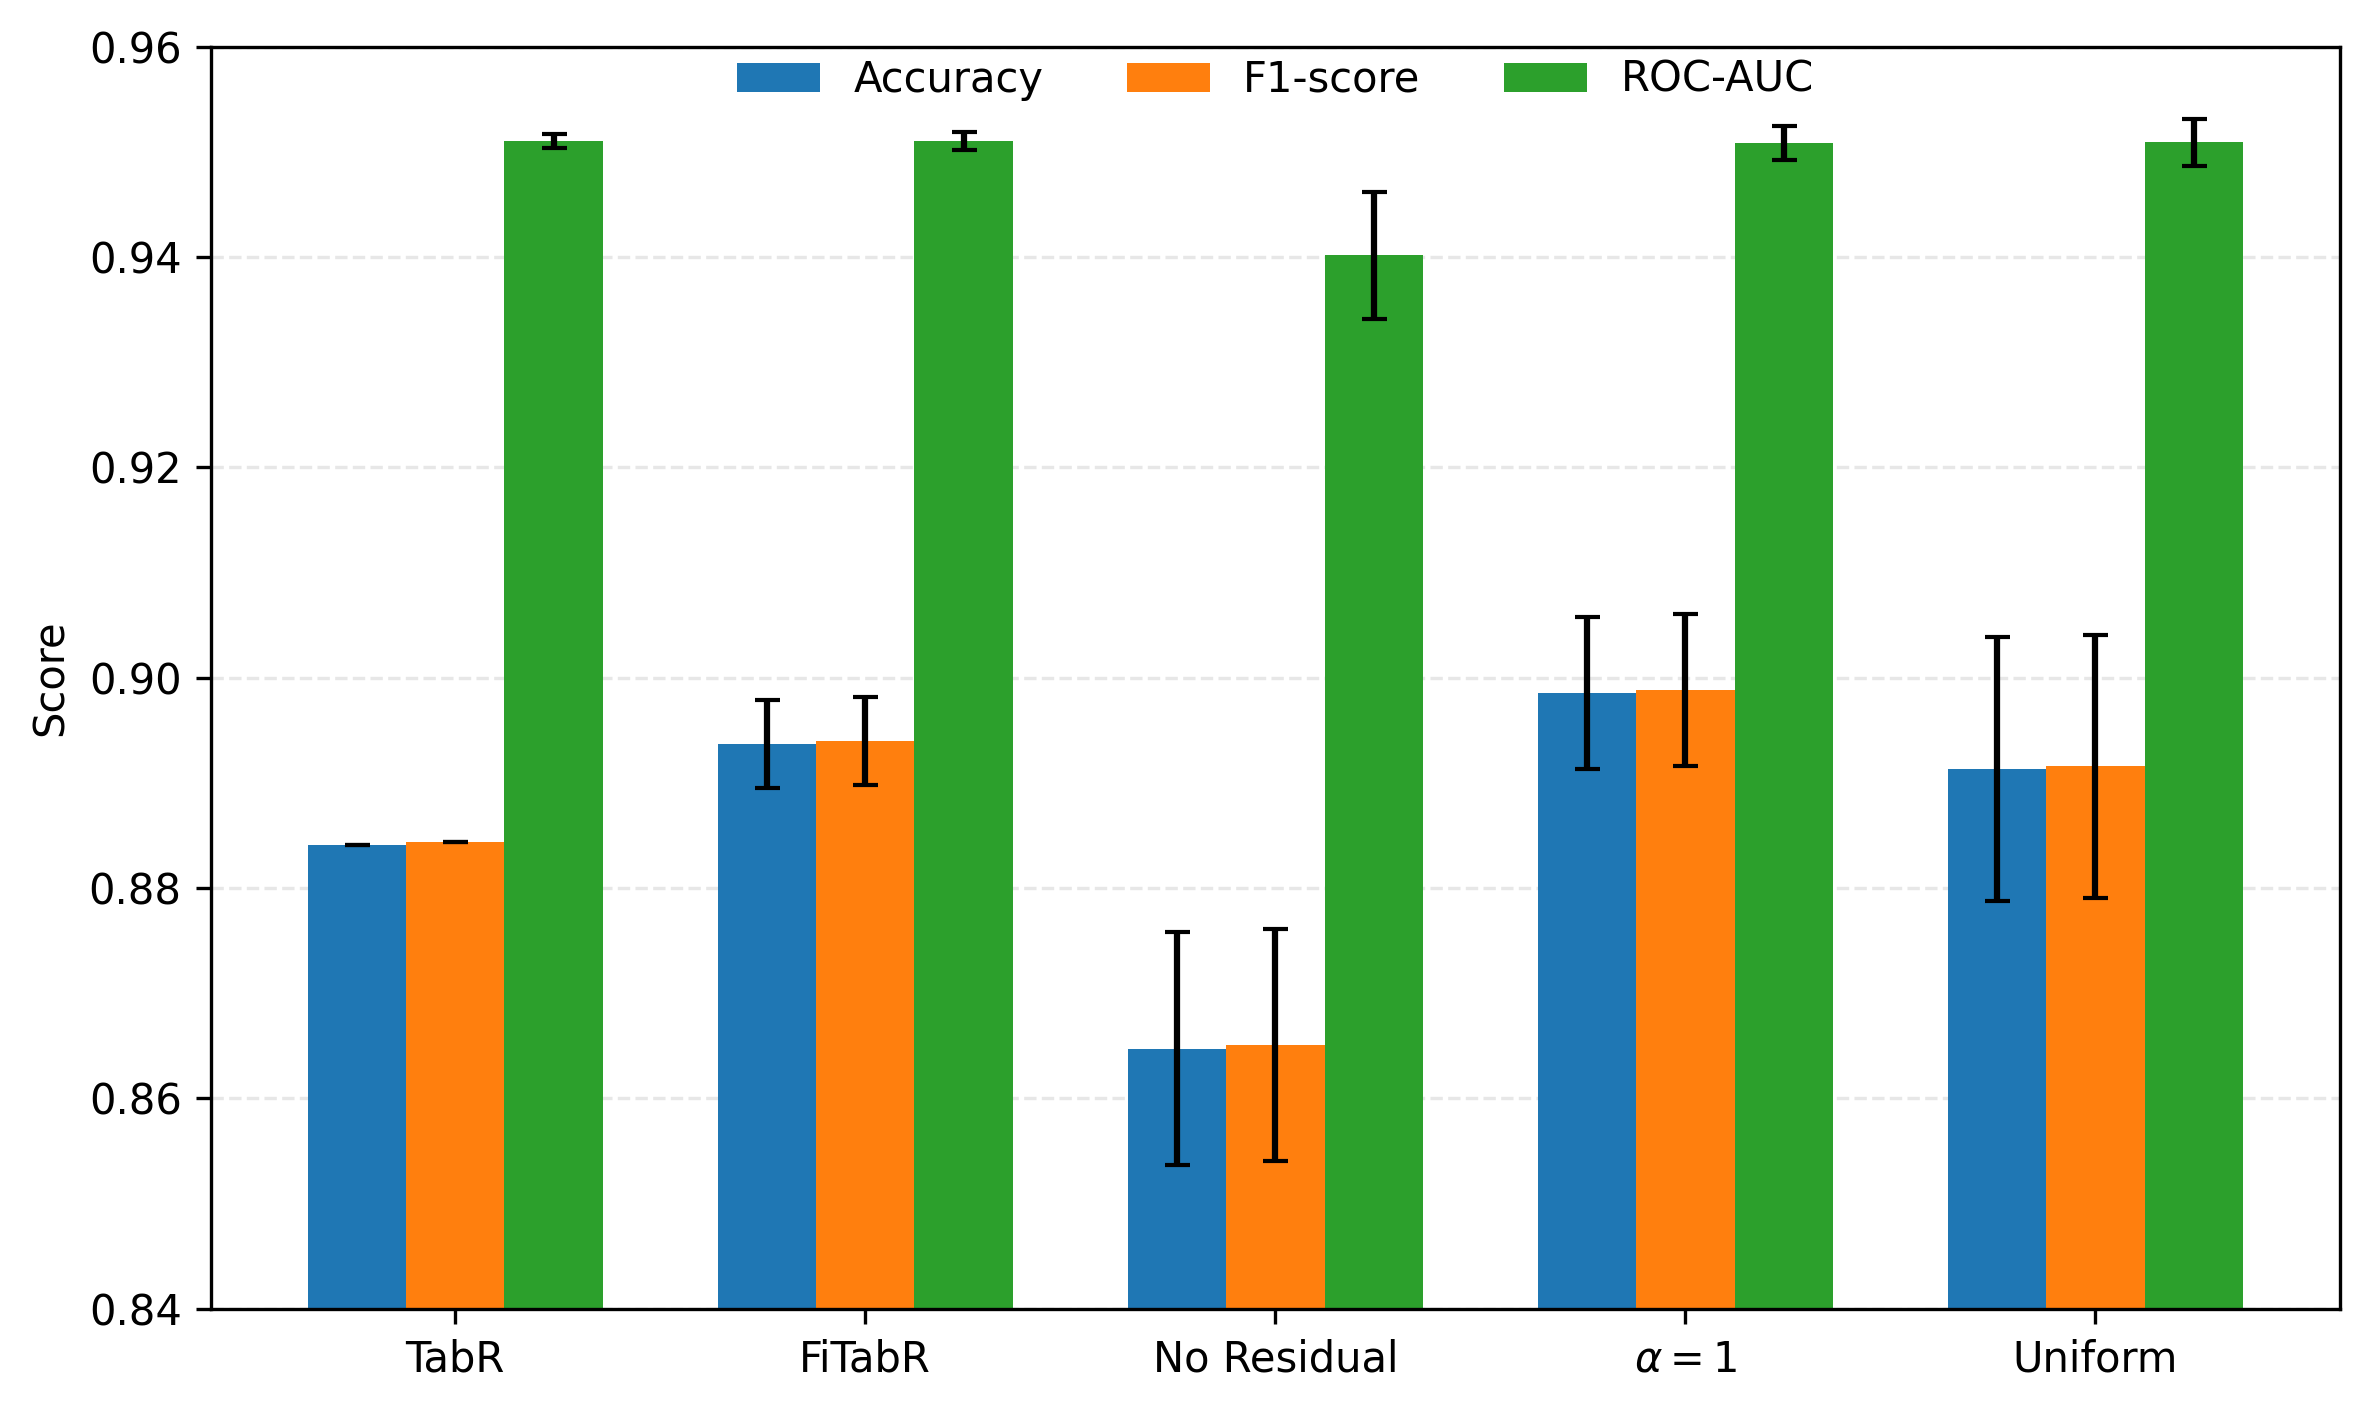
\includegraphics[width=0.80\textwidth]
    {figure/heart_ablation_performance.png}
    \caption{Ablation performance on the Heart Disease dataset.\\}
    \label{fig:heart_ablation_performance}
\end{figure}



% ============================================================
% Pima Diabetes
% ============================================================

\subsection{Pima Diabetes}
\label{subsec:pima_ablation}

Table~\ref{tab:pima_ablation} presents the corresponding ablation
results on the Pima Diabetes dataset.

\begin{table}[t]
\centering
\caption{Ablation study on the Pima Diabetes dataset. Results are
reported as mean $\pm$ standard deviation across three five-model
ensembles.\\}
\label{tab:pima_ablation}

\resizebox{\textwidth}{!}{
\begin{tabular}{lccc|cccc}
\toprule
Model &
Learned $a_i$ &
Residual &
$\alpha=2$ &
Acc. $\uparrow$ &
F1 $\uparrow$ &
AUC $\uparrow$ &
CE $\downarrow$
\\
\midrule

TabR
& $\times$
& $\times$
& $\times$
& 0.7529 $\pm$ 0.0050
& 0.7520 $\pm$ 0.0058
& 0.7963 $\pm$ 0.0072
& 0.5511 $\pm$ 0.0120
\\

FiTabR
& $\checkmark$
& $\checkmark$
& $\checkmark$
& 0.7586 $\pm$ 0.0086
& 0.7589 $\pm$ 0.0092
& 0.7953 $\pm$ 0.0047
& 0.5474 $\pm$ 0.0044
\\

No Residual
& $\checkmark$
& $\times$
& $\checkmark$
& 0.7500 $\pm$ 0.0086
& 0.7469 $\pm$ 0.0082
& 0.7994 $\pm$ 0.0089
& 0.5254 $\pm$ 0.0165
\\

No Scale
& $\checkmark$
& $\checkmark$
& $\times$
& 0.7471 $\pm$ 0.0100
& 0.7467 $\pm$ 0.0104
& 0.7973 $\pm$ 0.0075
& 0.5393 $\pm$ 0.0187
\\

Uniform
& $\times$
& $\checkmark$
& $\checkmark$
& 0.7500 $\pm$ 0.0149
& 0.7501 $\pm$ 0.0132
& 0.7944 $\pm$ 0.0044
& 0.5501 $\pm$ 0.0086
\\

\bottomrule
\end{tabular}}
\end{table}

The differences between the Pima Diabetes configurations are
substantially smaller than those observed on Heart Disease. Relative to
TabR, complete FiTabR increases mean accuracy from $0.7529$ to $0.7586$
and weighted F1-score from $0.7520$ to $0.7589$, while cross-entropy
decreases from $0.5511$ to $0.5474$. In contrast, mean ROC-AUC changes
slightly from $0.7963$ to $0.7953$, so the result does not indicate an
improvement in ranking performance.

The ablated configurations are similarly close. No Residual obtains the
highest mean ROC-AUC ($0.7994$) and the lowest cross-entropy ($0.5254$),
while No Scale and Uniform remain close to the TabR baseline. In contrast
to Heart Disease, the experiment therefore does not identify one component
whose benefit is consistent across the reported metrics. The results
instead suggest that the effect of feature weighting is weaker and more
metric-dependent on this dataset.



Figure~\ref{fig:pima_ablation_performance} summarizes the corresponding ablation
comparison for Pima Diabetes.

\begin{figure}[H]
    \centering
    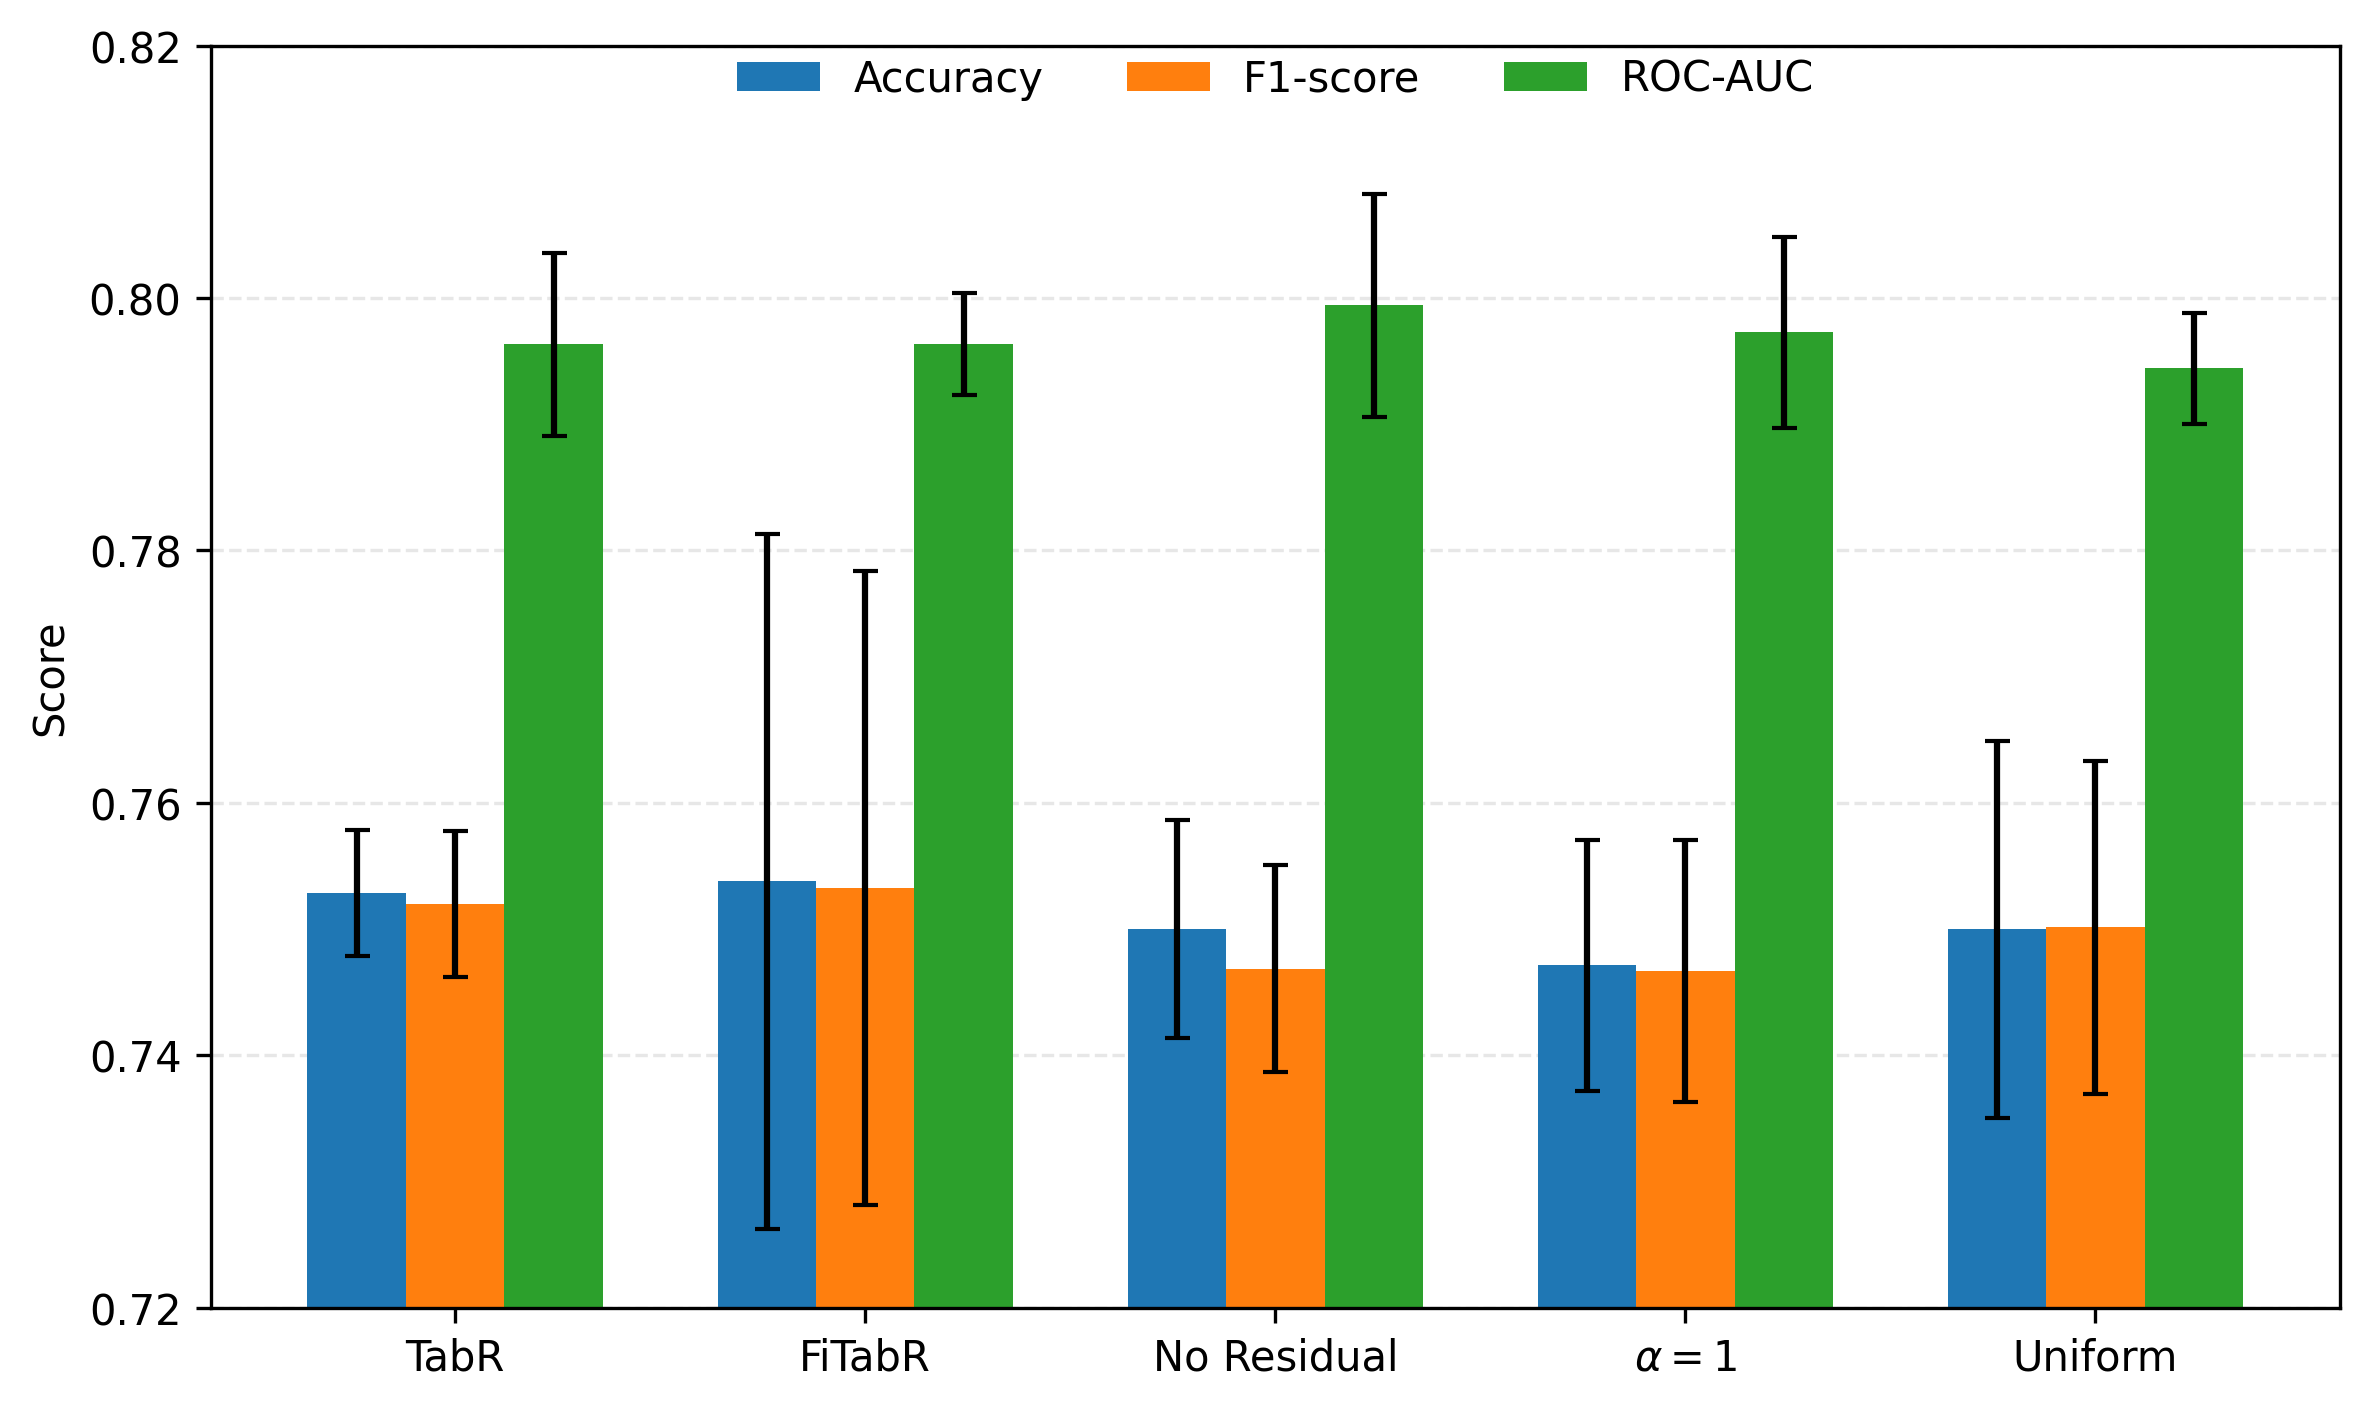
\includegraphics[width=0.90\textwidth]
    {figure/pima_ablation_performance.png}
    \caption{Ablation performance on the Pima Diabetes dataset.\\}
    \label{fig:pima_ablation_performance}
\end{figure}

% ============================================================
% Stroke Prediction
% ============================================================
\section{Stroke Prediction}
\label{subsec:stroke_ablation_performance}

Table~\ref{tab:stroke_ablation} reports the ablation results on the
Stroke Prediction dataset.

\begin{table}[t]
\centering
\caption{Ablation study on the Stroke Prediction dataset. Results are
reported as mean $\pm$ standard deviation across three five-model
ensembles.\\}
\label{tab:stroke_ablation}

\resizebox{\textwidth}{!}{
\begin{tabular}{lccc|cccc}
\toprule
Model &
Learned $a_i$ &
Residual &
$\alpha=2$ &
Acc. $\uparrow$ &
F1 $\uparrow$ &
AUC $\uparrow$ &
CE $\downarrow$
\\
\midrule

TabR
& $\times$
& $\times$
& $\times$
& 0.9505 $\pm$ 0.0000
& 0.9263 $\pm$ 0.0000
& 0.8136 $\pm$ 0.0078
& 0.1780 $\pm$ 0.0050
\\

FiTabR
& $\checkmark$
& $\checkmark$
& $\checkmark$
& 0.9505 $\pm$ 0.0000
& 0.9263 $\pm$ 0.0000
& 0.8095 $\pm$ 0.0126
& 0.1750 $\pm$ 0.0091
\\

No Residual
& $\checkmark$
& $\times$
& $\checkmark$
& 0.9505 $\pm$ 0.0000
& 0.9263 $\pm$ 0.0000
& 0.8104 $\pm$ 0.0089
& 0.1775 $\pm$ 0.0029
\\

No Scale
& $\checkmark$
& $\checkmark$
& $\times$
& 0.9505 $\pm$ 0.0000
& 0.9263 $\pm$ 0.0000
& 0.7985 $\pm$ 0.0053
& 0.1806 $\pm$ 0.0004
\\

Uniform
& $\times$
& $\checkmark$
& $\checkmark$
& 0.9505 $\pm$ 0.0000
& 0.9263 $\pm$ 0.0000
& 0.7727 $\pm$ 0.0363
& 0.1801 $\pm$ 0.0120
\\

\bottomrule
\end{tabular}
}
\end{table}

The threshold-based metrics are identical across all configurations on
the Stroke Prediction dataset. Consequently, accuracy and weighted
F1-score do not distinguish between the proposed feature-weighting
variants.

Differences are instead observed in probability-based metrics. TabR
obtains the highest mean ROC-AUC of $0.8136$, while complete FiTabR
obtains $0.8095$. No Residual remains close to both configurations at
$0.8104$. In contrast, removing the scaling coefficient reduces
ROC-AUC to $0.7985$, and replacing learned attention with uniform
weighting produces the largest deterioration, reaching $0.7727$.

Complete FiTabR obtains the lowest mean cross-entropy, decreasing from
$0.1780$ for TabR to $0.1750$. However, this improvement in
probabilistic fit does not correspond to an improvement in ROC-AUC or
threshold-based classification performance.

Thus, unlike Heart Disease, the Stroke Prediction experiment does not
provide evidence that feature-aware weighting improves overall
discrimination. The result also illustrates that weighted
threshold-based metrics can conceal differences between models on a
strongly imbalanced dataset.



Figure~\ref{fig:figure/stroke_ablation_performance} visualizes the ablation results on the
Stroke Prediction dataset.

\begin{figure}[H]
    \centering
    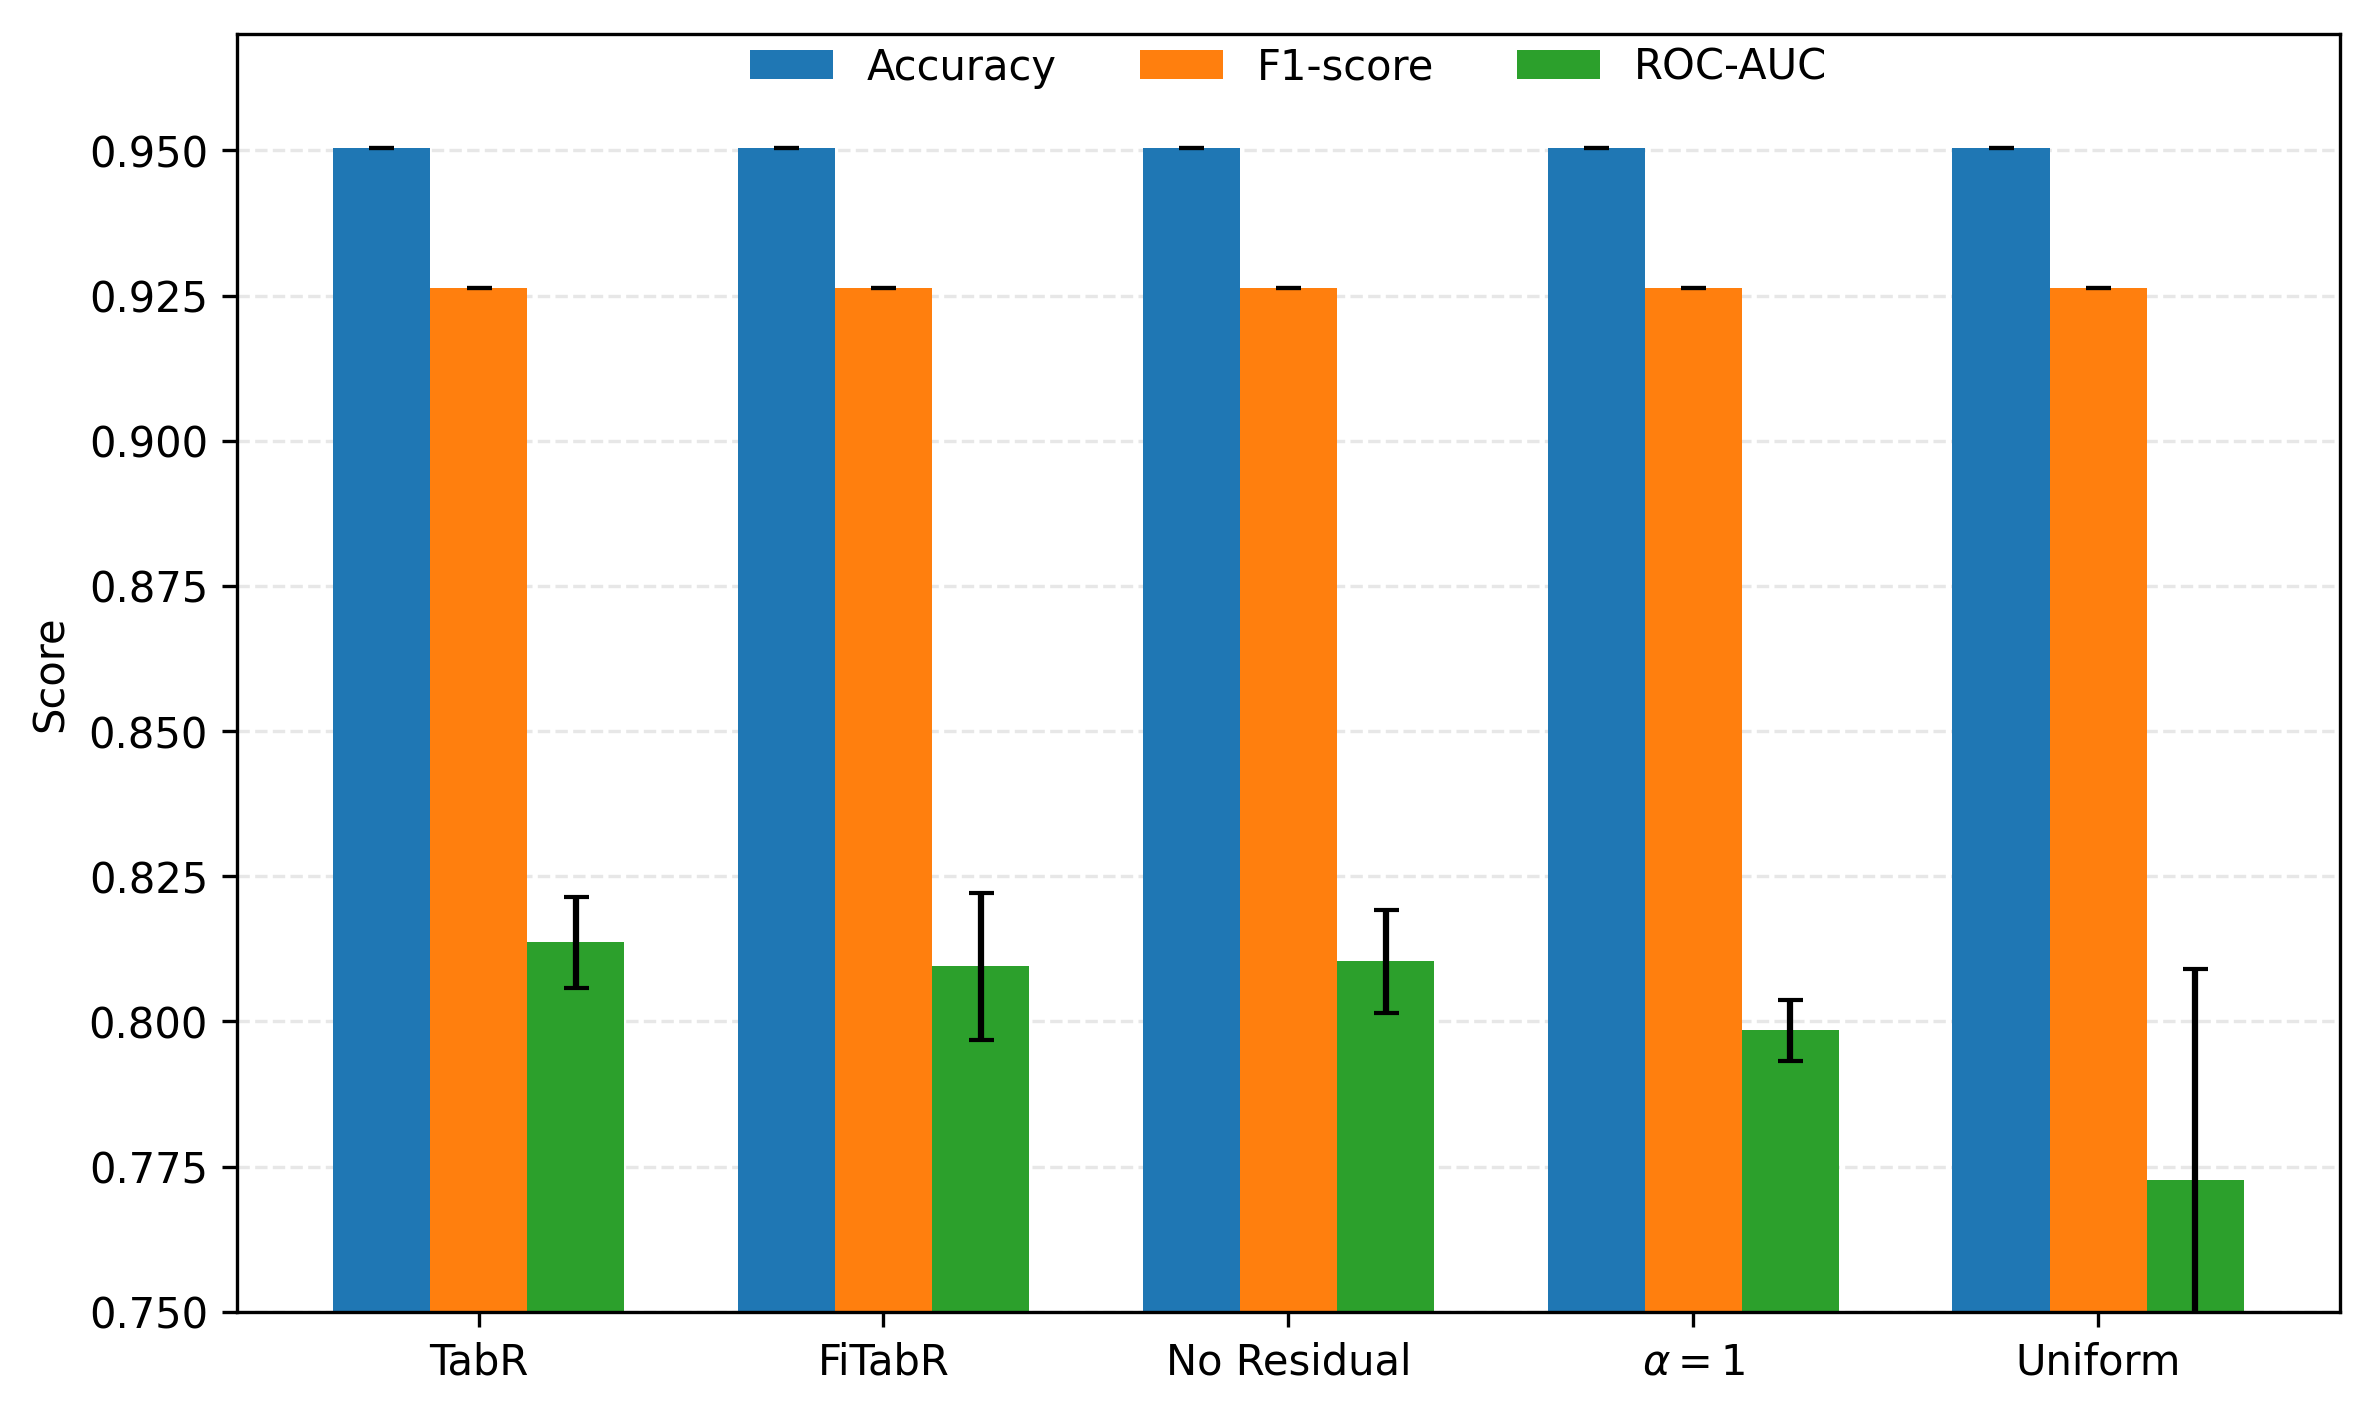
\includegraphics[width=0.80\textwidth]
    {figure/stroke_ablation_performance.png}
    \caption{Ablation performance on the Stroke Prediction dataset. }
    \label{fig:stroke_ablation_performance}
\end{figure}

% ============================================================
% Overall Discussion
% ============================================================

\subsection{Discussion}
\label{subsec:ablation_discussion}

Overall, the ablation study shows that the effect of the FiTabR
components depends strongly on the dataset. The clearest result is
observed on Heart Disease. On this dataset, complete FiTabR improves over
TabR, whereas removing residual feature weighting causes a substantial
performance drop. This provides evidence that preserving the original
numerical representation while applying feature-dependent modulation is
important for the proposed approach.

The results provide weaker support for the fixed scaling coefficient.
The No Scale configuration remains competitive with, and is numerically
slightly better than, complete FiTabR on Heart Disease. Since the
difference is small relative to the reported ensemble variation, the
experiment does not establish that $\alpha=2.0$ is preferable to using
the unscaled attention distribution.

The Uniform variant provides an additional control for the learned
attention mechanism. Its competitive performance on Heart Disease
indicates that numerical feature modulation itself may account for part
of the observed improvement. However, its substantially lower ROC-AUC
on Stroke Prediction shows that uniform reweighting is not consistently
beneficial across datasets.

Pima Diabetes shows only small differences between the configurations,
while Stroke Prediction shows no improvement in threshold-based
classification performance. Therefore, the ablation results do not
support a claim that the complete FiTabR configuration is universally
superior to TabR.

Instead, the experiments indicate that explicit pre-retrieval feature
reweighting can be beneficial under some dataset conditions, with the
strongest evidence obtained on Heart Disease. Among the examined design
choices, residual feature preservation receives the clearest empirical
support, while the contribution of fixed attention scaling and learned
sample-specific weighting is more dataset-dependent.

\section{Clinical Concordance of Learned Feature Attention}
\label{sec:clinical_attention}

Attention-based tabular models such as TabNet use learned feature-selection
signals to expose aspects of model behavior \cite{arik2021tabnet}. However,
attention weights should not automatically be interpreted as faithful
explanations of predictions \cite{jain2019attention}. Accordingly, the
analysis in this section is restricted to qualitative clinical concordance.
FiTabR attention is treated as model-internal feature emphasis rather than a
causal effect, clinical risk coefficient, or direct measure of medical
importance.

The mean feature-attention values are compared with established domain
knowledge from cardiovascular, diabetes, and stroke guidelines, the
Framingham studies, and large prospective meta-analyses
\cite{visseren2021,dagostino2008,score2_2021,ctt2012,erfc2010,
ada2026diagnosis,bushnell2024}. The attention statistics correspond to the
selected FiTabR models recorded in the experiment reports.

\subsection{Heart Disease}
\label{subsec:heart_attention}

The Heart Disease results show partial agreement between the learned FiTabR
attention distribution and established cardiovascular knowledge. Cholesterol
and age receive the two highest mean attention values and are also
well-established cardiovascular risk-related variables. Resting blood pressure
receives intermediate attention despite its strong clinical importance, while
Oldpeak and maximum heart rate receive lower attention despite their known
prognostic value.

The relatively large standard deviation of cholesterol attention
($0.1155$) indicates that FiTabR does not emphasize this feature equally for
every sample. Instead, its contribution to the learned representation varies
across patient profiles. Figure~\ref{fig:heart_attention} compares the learned
mean attention values with the uniform-attention reference.

\begin{figure}[htbp]
    \centering
    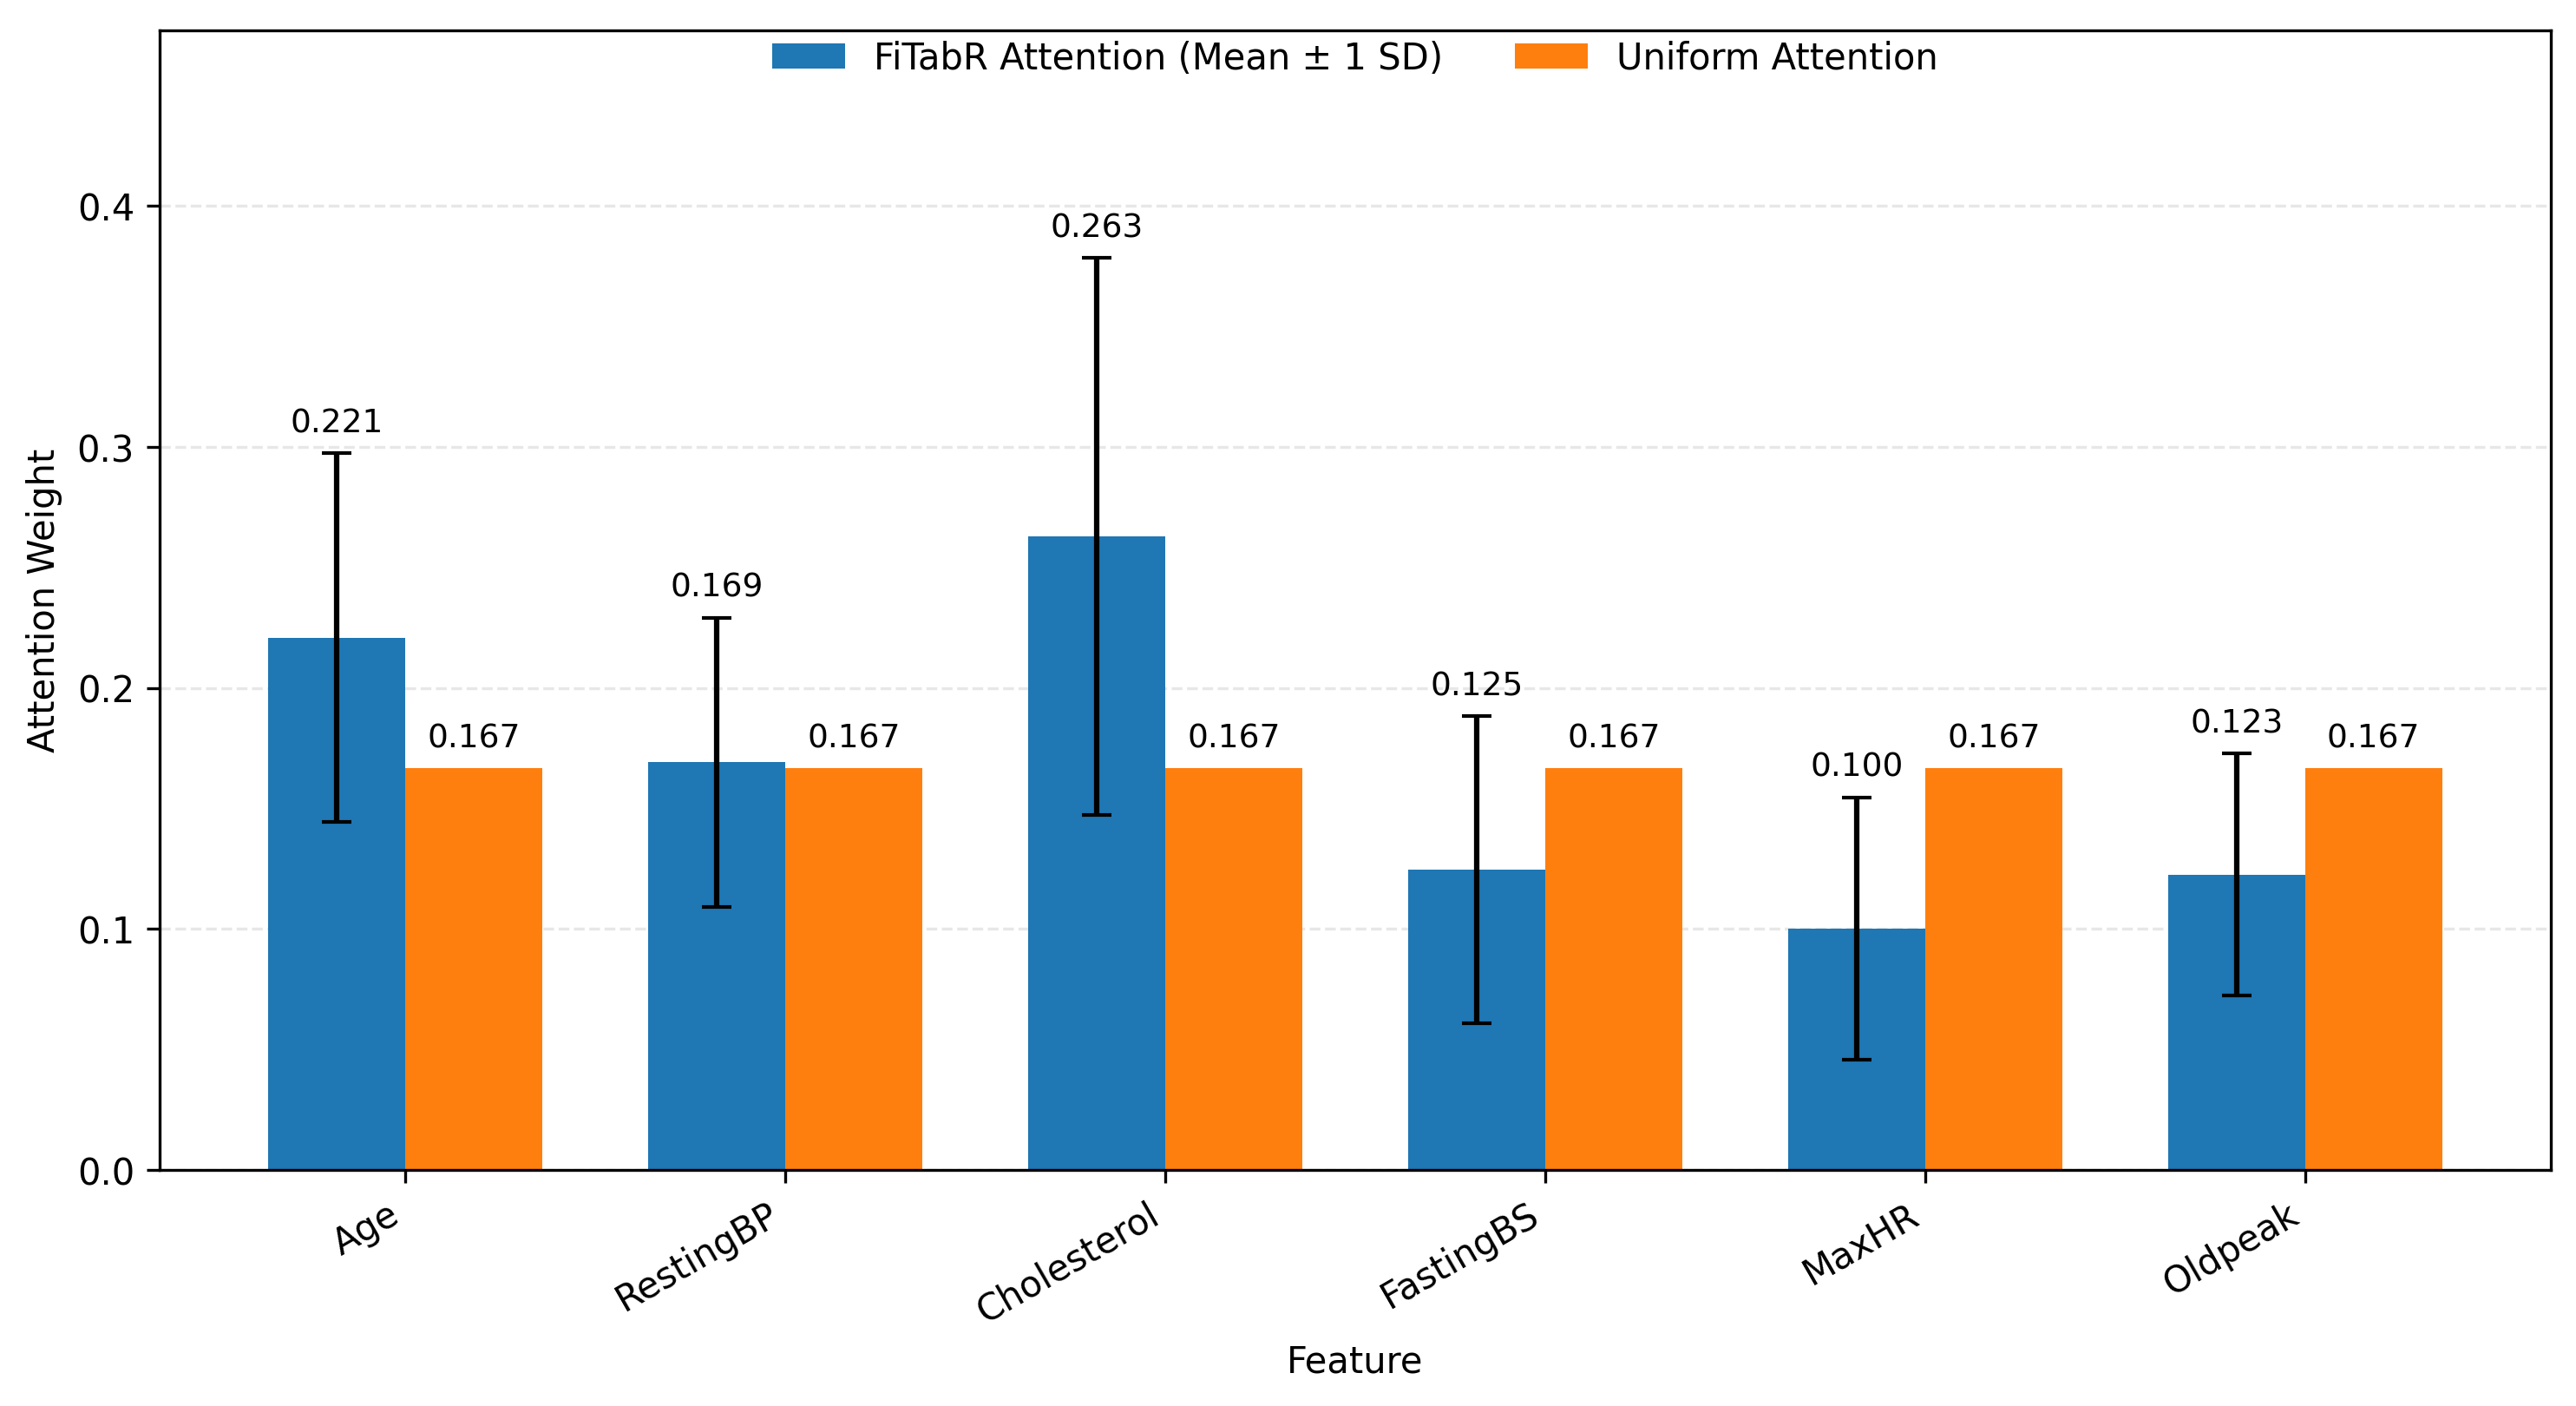
\includegraphics[width=0.92\textwidth]
    {figure/heart_attention_analysis.png}
    \caption{FiTabR feature-attention distribution on the Heart Disease
    dataset. Learned bars show mean attention with $\pm 1$ standard deviation;
    uniform bars show the reference value $1/F$ for each numerical feature.}
    \label{fig:heart_attention}
\end{figure}

\begin{table}[H]
\centering
\caption{Comparison of FiTabR attention with established cardiovascular
domain knowledge on the Heart Disease dataset.\\}
\label{tab:heart_attention_domain}
\renewcommand{\arraystretch}{1.20}
\setlength{\tabcolsep}{5pt}
\small

\begin{tabularx}{\textwidth}{
    >{\raggedright\arraybackslash}p{2.2cm}
    >{\centering\arraybackslash}p{2.7cm}
    X}

\toprule
\textbf{Feature} &
\textbf{Attention Mean $\pm$ SD} &
\textbf{Established Clinical Context} \\
\midrule

Cholesterol &
$\mathbf{0.2627 \pm 0.1155}$ &
Major contributor to atherosclerotic cardiovascular risk
\cite{ctt2012,visseren2021}. \\

Age &
$\mathbf{0.2208 \pm 0.0765}$ &
Major cardiovascular risk determinant included in established
risk-prediction models \cite{dagostino2008,score2_2021}. \\

RestingBP &
$0.1691 \pm 0.0600$ &
Elevated blood pressure is a major modifiable cardiovascular
risk factor \cite{lewington2002,visseren2021}. \\

FastingBS &
$0.1246 \pm 0.0637$ &
Diabetes and elevated glucose are associated with increased
cardiovascular risk \cite{erfc2010}. \\

Oldpeak &
$0.1226 \pm 0.0502$ &
Exercise-induced ST-segment deviation has established diagnostic
and prognostic relevance \cite{mark1991}. \\

MaxHR &
$0.1002 \pm 0.0544$ &
Impaired exercise heart-rate response is associated with adverse
cardiovascular outcomes \cite{lauer1996}. \\

\bottomrule
\end{tabularx}
\end{table}

Overall, the Heart Disease attention pattern is medically plausible in part,
but it should not be interpreted as a conventional cardiovascular risk-factor
ranking.

\subsection{Pima Diabetes}
\label{subsec:pima_attention}

The Pima Diabetes results demonstrate partial clinical concordance.
SkinThickness receives the highest mean attention, followed by insulin, BMI,
and age. These variables are related to adiposity, insulin regulation, and
metabolic risk, which are important components of Type 2 diabetes development.
The relatively large standard deviation of insulin attention ($0.1157$)
further indicates substantial variation in its model-internal emphasis across
individual samples.

The most notable discrepancy is glucose. Although glucose measurements are
central to diabetes screening and diagnosis, glucose receives relatively low
mean FiTabR attention. BloodPressure and DiabetesPedigreeFunction also receive
low attention despite their associations with cardiometabolic and familial
risk. Figure~\ref{fig:pima_attention} shows the learned attention distribution
against the corresponding uniform reference.

\begin{figure}[htbp]
    \centering
    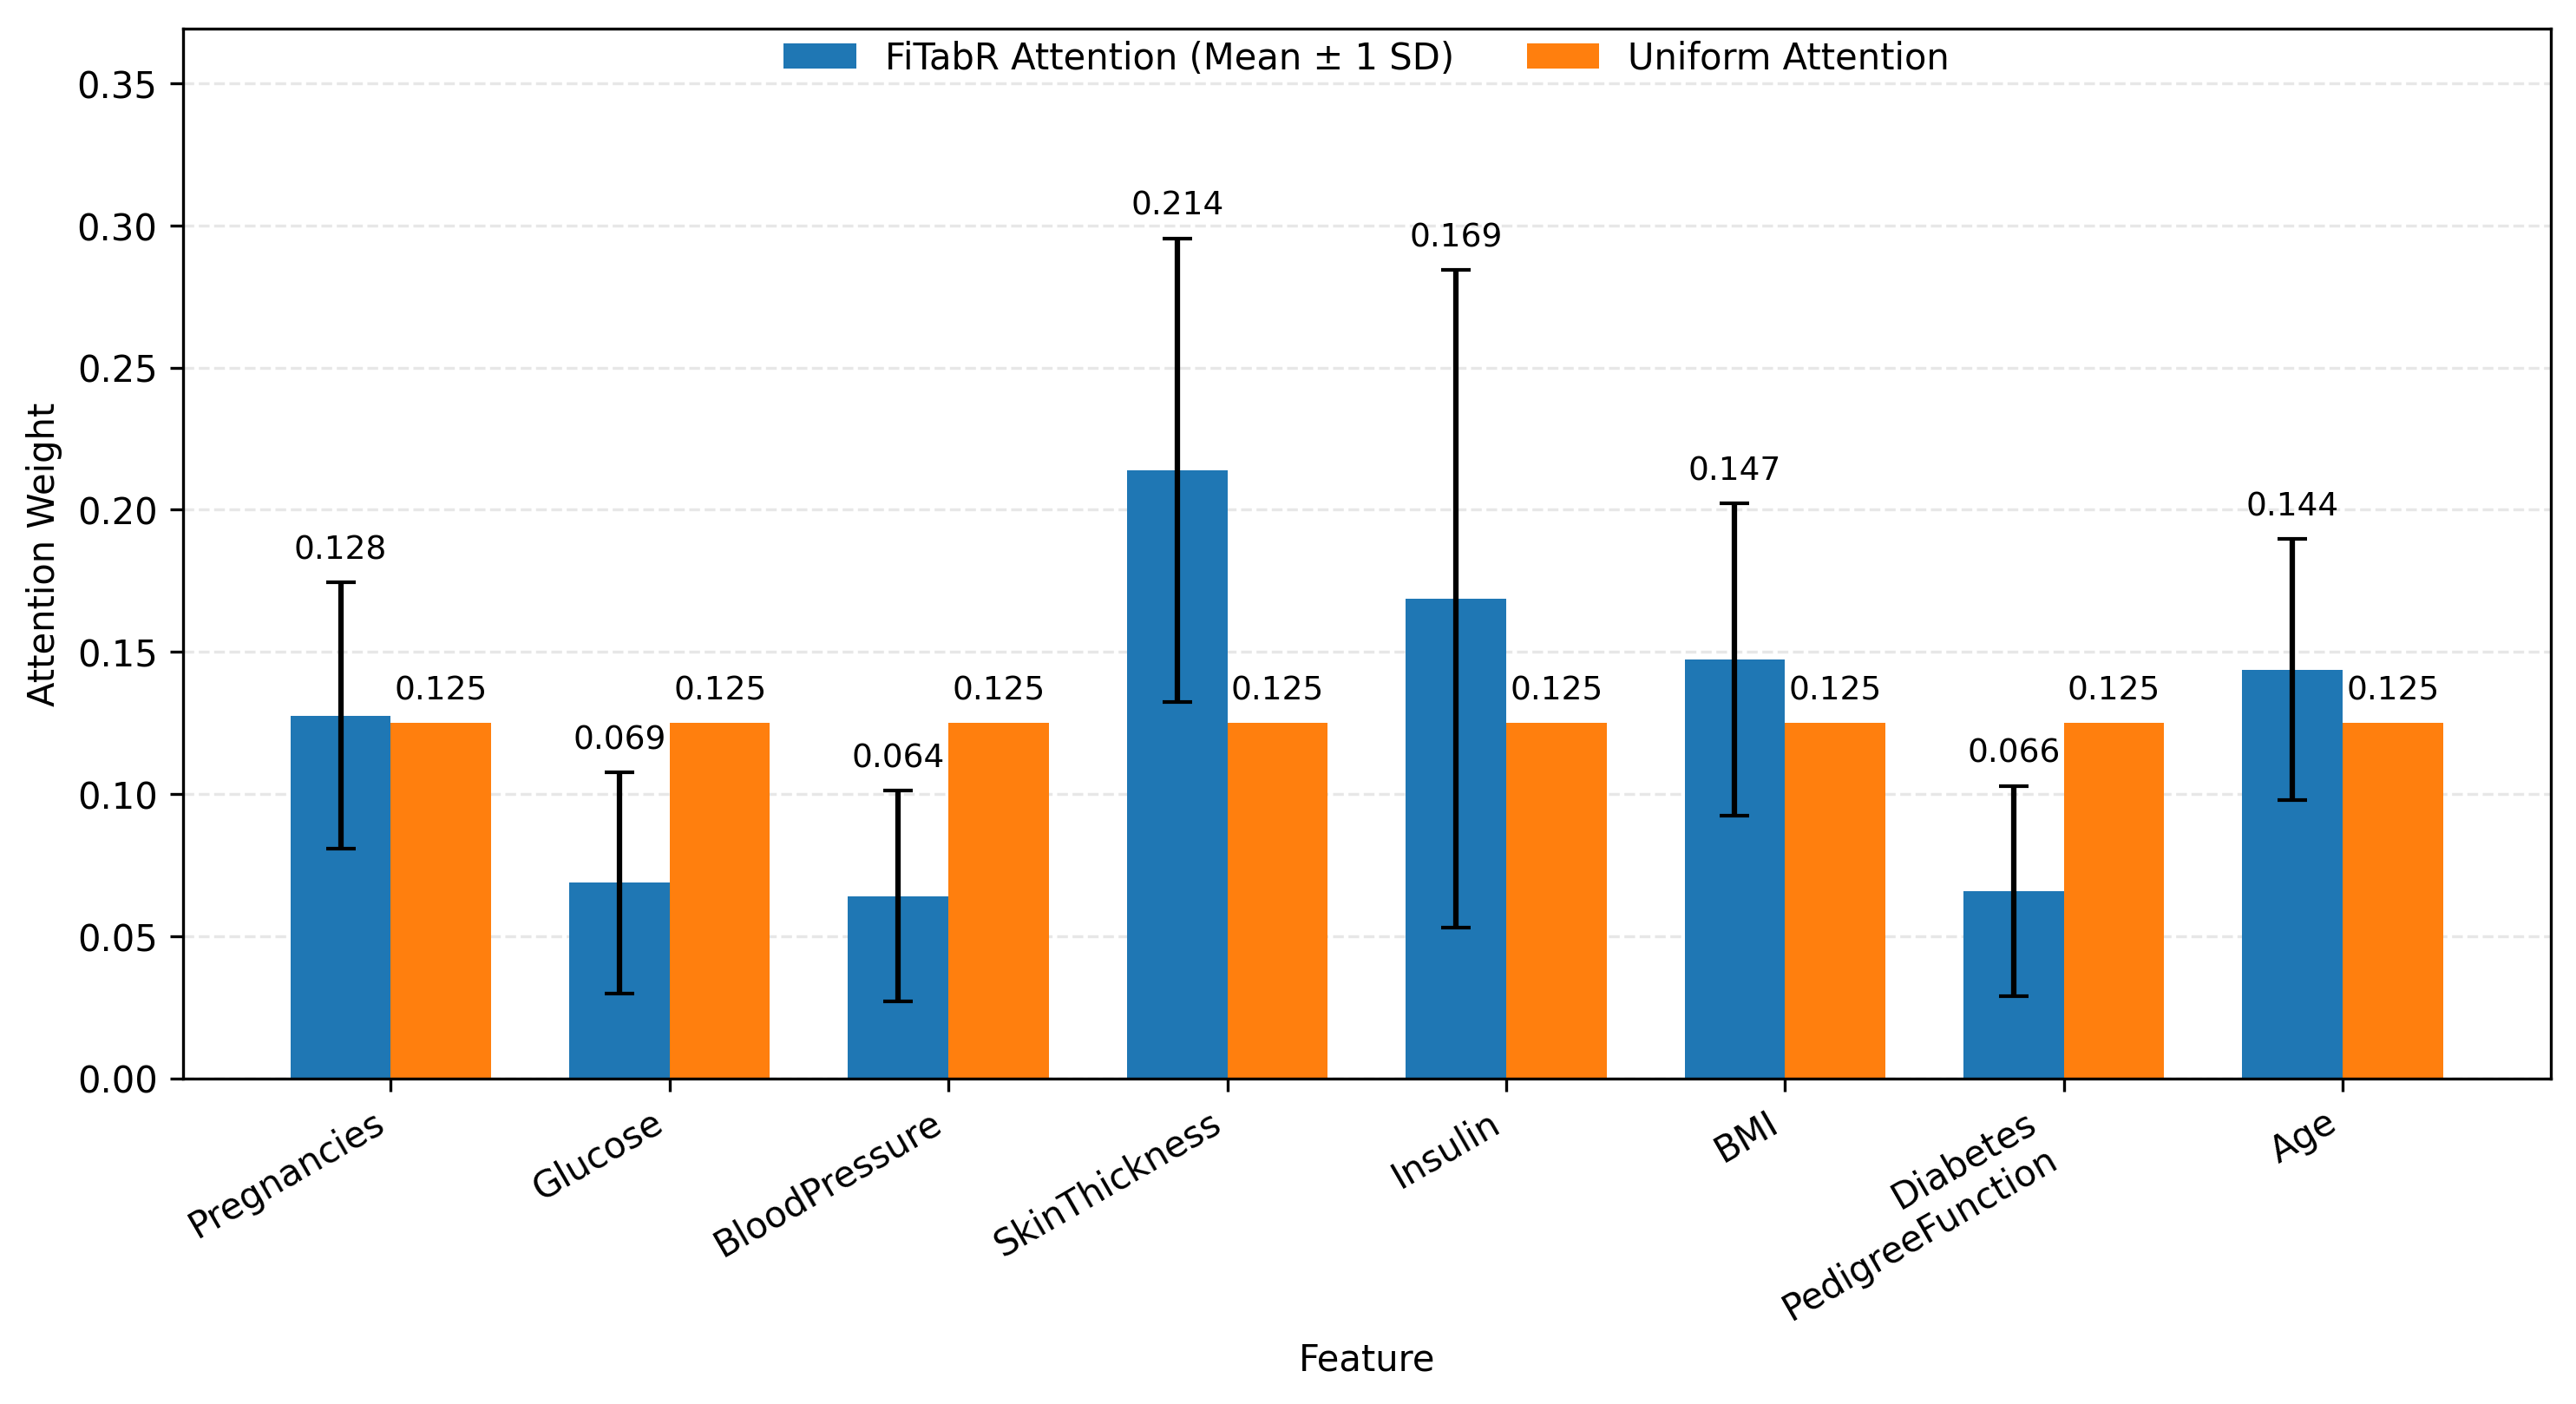
\includegraphics[width=0.92\textwidth]
    {figure/pima_attention_analysis.png}
    \caption{FiTabR feature-attention distribution on the Pima Diabetes
    dataset. Learned bars show mean attention with $\pm 1$ standard deviation;
    uniform bars show the reference value $1/F$ for each numerical feature.}
    \label{fig:pima_attention}
\end{figure}

\begin{table}[H]
\centering
\caption{Comparison of FiTabR attention with established medical
domain knowledge on the Pima Diabetes dataset.\\}
\label{tab:pima_attention_domain}
\renewcommand{\arraystretch}{1.20}
\setlength{\tabcolsep}{5pt}
\small

\begin{tabularx}{\textwidth}{
    >{\raggedright\arraybackslash}p{2.7cm}
    >{\centering\arraybackslash}p{2.7cm}
    X}

\toprule
\textbf{Feature} &
\textbf{Attention Mean $\pm$ SD} &
\textbf{Established Clinical Context} \\
\midrule

SkinThickness &
$\mathbf{0.2139 \pm 0.0816}$ &
Indicator of subcutaneous adiposity associated with insulin
resistance and Type 2 diabetes risk
\cite{sosenko1993,ada2026obesity}. \\

Insulin &
$\mathbf{0.1687 \pm 0.1157}$ &
Insulin resistance and $\beta$-cell dysfunction are central to
Type 2 diabetes pathophysiology \cite{defronzo2009}. \\

BMI &
$0.1474 \pm 0.0548$ &
Overweight and obesity are established Type 2 diabetes risk
factors \cite{ada2026diagnosis,ada2026obesity}. \\

Age &
$0.1438 \pm 0.0459$ &
Increasing age is an established diabetes risk factor used in
screening recommendations \cite{ada2026diagnosis}. \\

Pregnancies &
$0.1276 \pm 0.0469$ &
Pregnancy-related metabolic history can be associated with
future diabetes risk \cite{ada2026diagnosis}. \\

Glucose &
$0.0688 \pm 0.0389$ &
Glucose measurement is central to diabetes screening and
diagnosis \cite{ada2026diagnosis}. \\

DiabetesPedigreeFunction &
$0.0658 \pm 0.0370$ &
Represents familial predisposition; family history is an
established diabetes risk factor \cite{ada2026diagnosis}. \\

BloodPressure &
$\mathbf{0.0641 \pm 0.0370}$ &
Hypertension is associated with cardiometabolic and diabetes
risk \cite{ada2026diagnosis}. \\

\bottomrule
\end{tabularx}
\end{table}

The discrepancy between model attention and established clinical relevance,
especially for glucose, reinforces that FiTabR attention is a property of the
learned representation rather than a direct ranking of diabetes risk factors.

\subsection{Stroke Prediction}
\label{subsec:stroke_attention}

The Stroke results also demonstrate partial clinical concordance. Average
glucose level and age receive the two largest attention values, consistent
with established evidence linking diabetes, hyperglycemia, increasing age,
and stroke risk. The relatively large standard deviation of glucose attention
($0.1262$) further indicates substantial variation in its model-internal
emphasis across individual samples.

The most notable discrepancy is hypertension. Although hypertension is one of
the strongest established modifiable risk factors for stroke, it receives the
lowest mean FiTabR attention. The binary hypertension variable contains less
information than a continuous blood-pressure measurement, and the model may
also represent correlated information through age, glucose, BMI,
cardiovascular history, and other features. Figure~\ref{fig:stroke_attention}
visualizes this feature-emphasis pattern.

\begin{figure}[htbp]
    \centering
    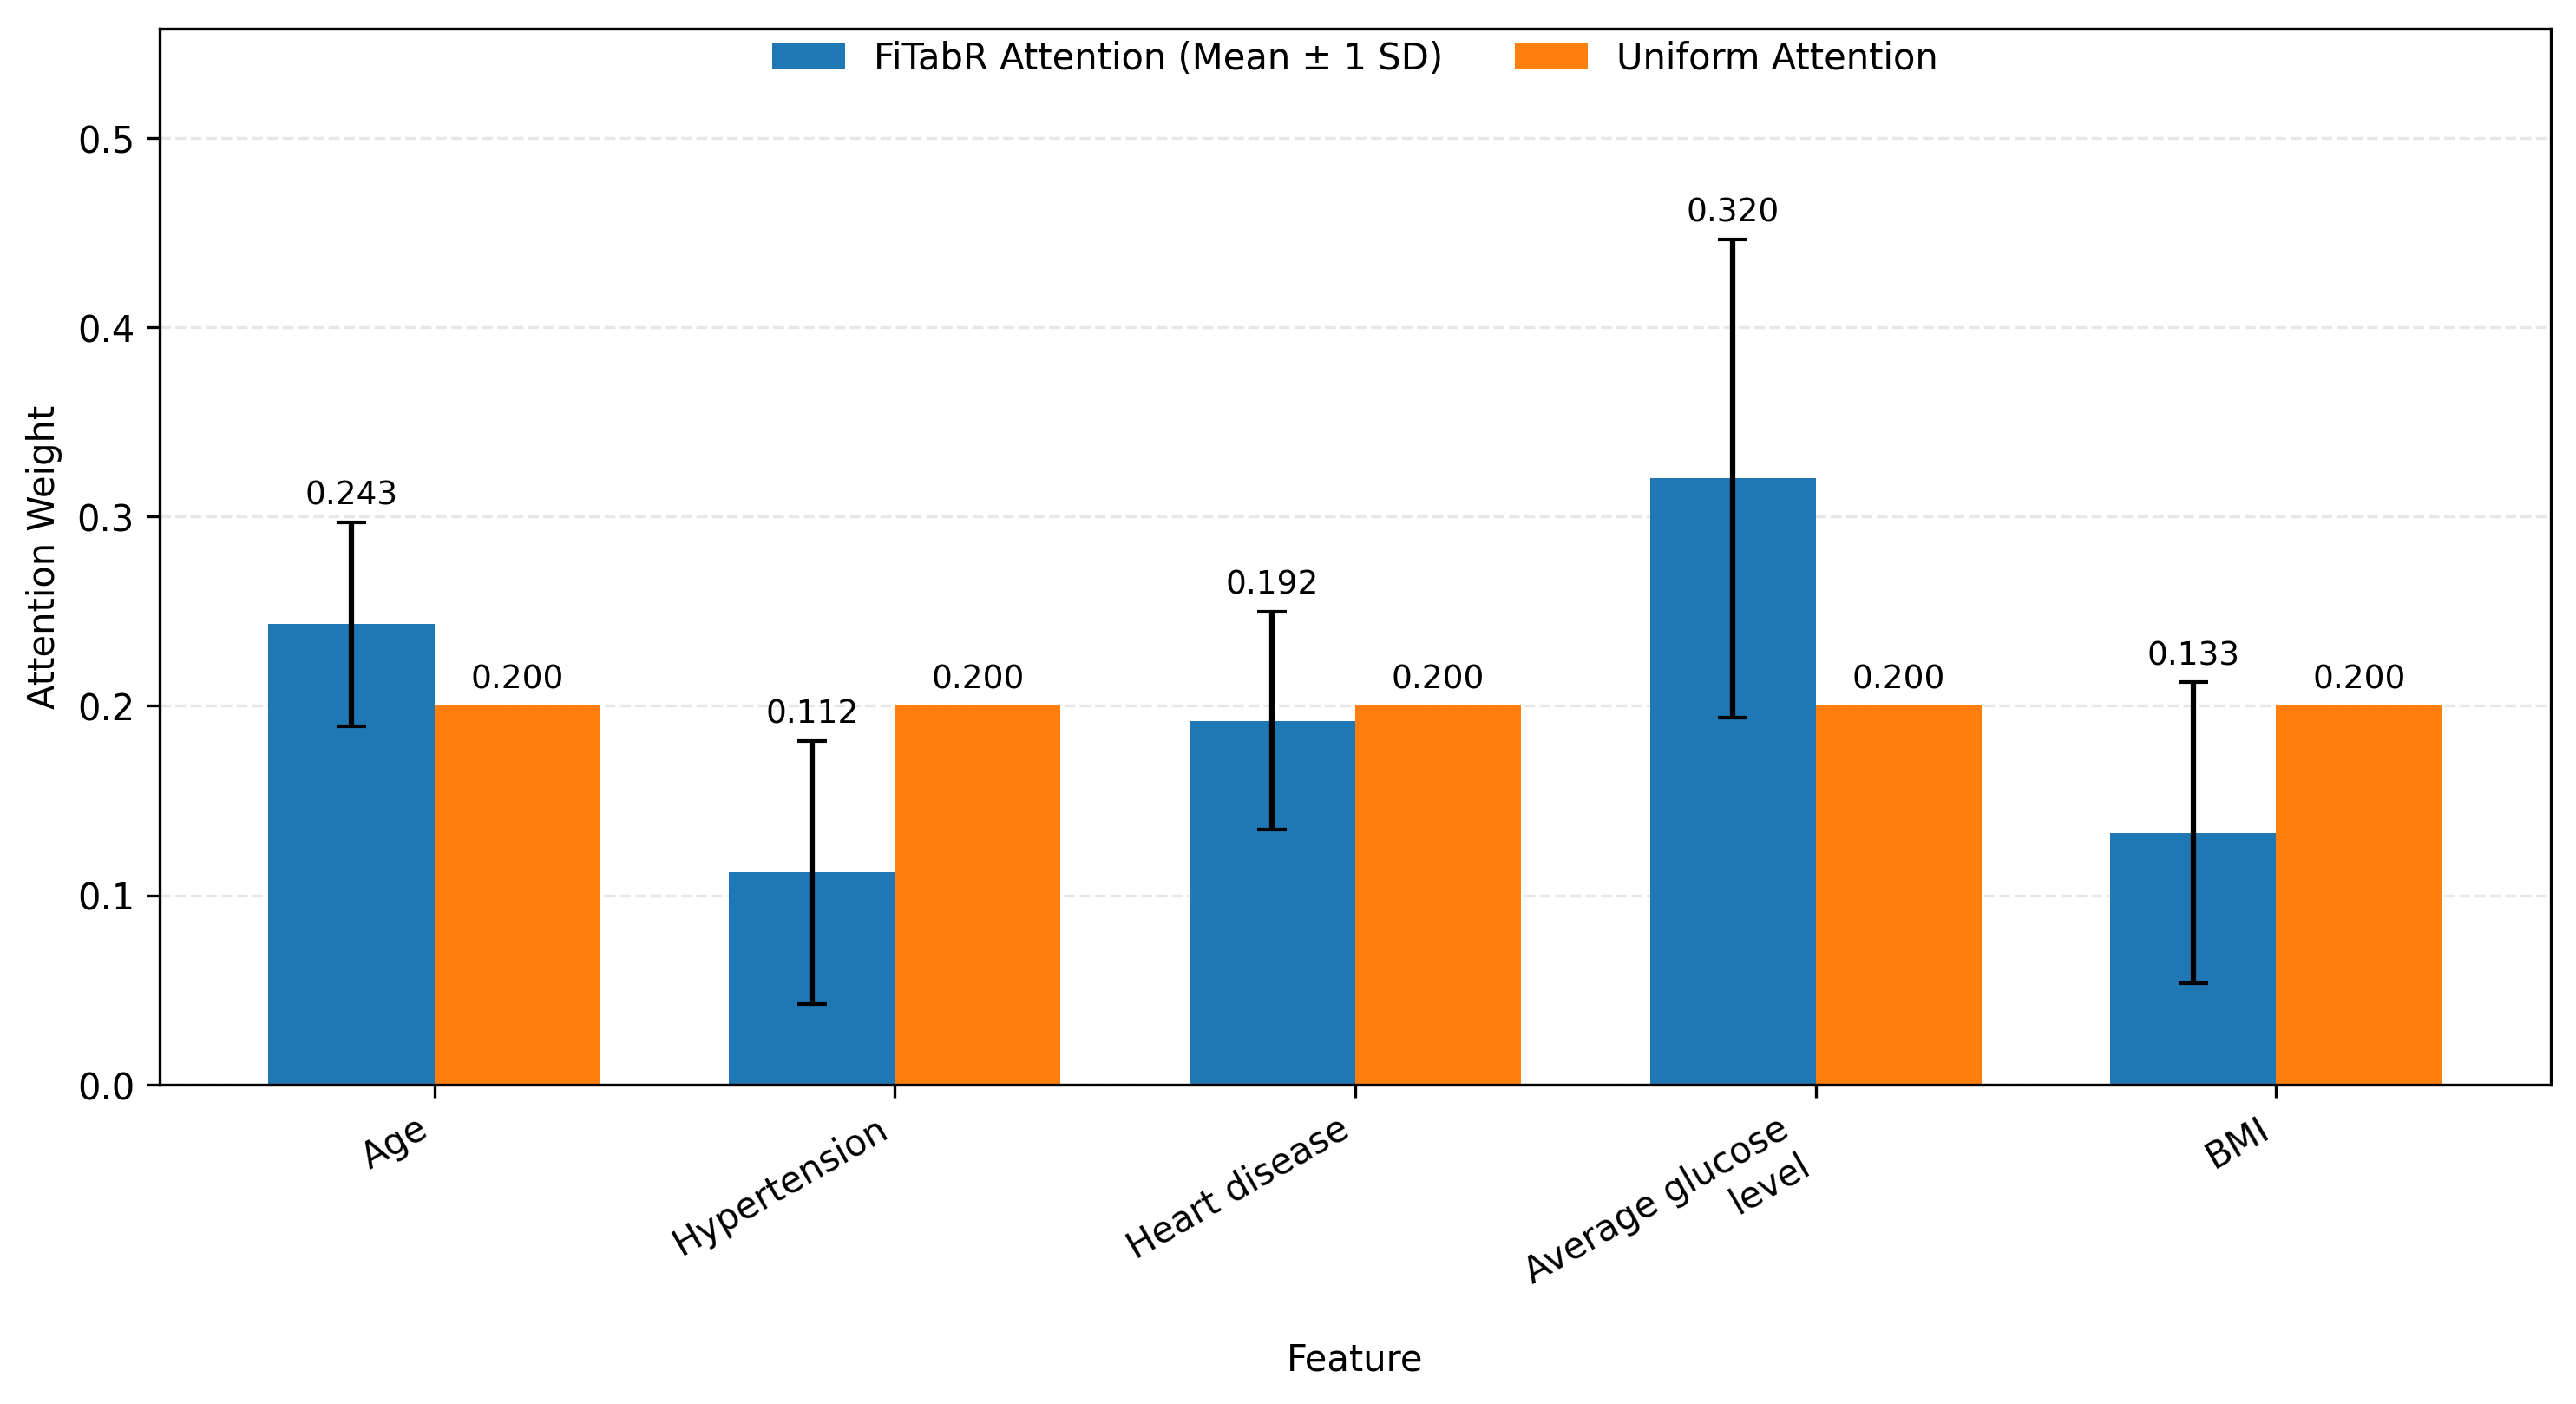
\includegraphics[width=0.92\textwidth]
    {figure/stroke_attention_analysis.png}
    \caption{FiTabR feature-attention distribution on the Stroke Prediction
    dataset. Learned bars show mean attention with $\pm 1$ standard deviation;
    uniform bars show the reference value $1/F$ for each numerical feature.}
    \label{fig:stroke_attention}
\end{figure}

\begin{table}[H]
\centering
\caption{Comparison of FiTabR attention with established medical
domain knowledge on the Stroke Prediction dataset.\\}
\label{tab:stroke_attention_domain}
\renewcommand{\arraystretch}{1.20}
\setlength{\tabcolsep}{5pt}
\small

\begin{tabularx}{\textwidth}{
    >{\raggedright\arraybackslash}p{2.5cm}
    >{\centering\arraybackslash}p{2.7cm}
    X}

\toprule
\textbf{Feature} &
\textbf{Attention Mean $\pm$ SD} &
\textbf{Established Clinical Context} \\
\midrule

Average glucose level &
$\mathbf{0.3200 \pm 0.1262}$ &
Diabetes and hyperglycemia are established stroke risk factors
\cite{erfc2010,bushnell2024}. \\

Age &
$\mathbf{0.2430 \pm 0.0540}$ &
Major non-modifiable determinant of stroke risk
\cite{wolf1991}. \\

Heart disease &
$0.1920 \pm 0.0576$ &
Cardiovascular disease is associated with increased stroke risk
\cite{kannel1983}. \\

BMI &
$0.1329 \pm 0.0794$ &
Higher BMI is associated with stroke risk, partly through
metabolic risk factors \cite{gbd2014}. \\

Hypertension &
$\mathbf{0.1121 \pm 0.0695}$ &
Major modifiable stroke risk factor and prevention target
\cite{bushnell2024,lewington2002}. \\

\bottomrule
\end{tabularx}
\end{table}
\subsection{Attention Analysis Summary}

Across the three datasets, FiTabR learns several attention patterns that are
consistent with established medical knowledge: cholesterol and age receive the
largest mean attention on Heart Disease, SkinThickness, insulin, BMI, and age
receive comparatively high attention on Pima Diabetes, and average glucose
level and age receive the largest attention on Stroke Prediction.

At the same time, clinically meaningful discrepancies remain. Glucose receives
relatively low attention on Pima Diabetes despite its central diagnostic role,
and hypertension receives the lowest mean attention on Stroke Prediction
despite being an established modifiable stroke-risk factor. These findings
support interpreting FiTabR attention as model-specific feature emphasis, not
as epidemiological, causal, or clinical risk estimates.



    
    
    \section{Some Common Mistakes}\label{SCM}
    \begin{itemize}
    \item The word ``data'' is plural, not singular.
    \item The subscript for the permeability of vacuum $\mu_{0}$, and other common scientific constants, is zero with subscript formatting, not a lowercase letter ``o''.
    \item In American English, commas, semicolons, periods, question and exclamation marks are located within quotation marks only when a complete thought or name is cited, such as a title or full quotation. When quotation marks are used, instead of a bold or italic typeface, to highlight a word or phrase, punctuation should appear outside of the quotation marks. A parenthetical phrase or statement at the end of a sentence is punctuated outside of the closing parenthesis (like this). (A parenthetical sentence is punctuated within the parentheses.)
    \item A graph within a graph is an ``inset'', not an ``insert''. The word alternatively is preferred to the word ``alternately'' (unless you really mean something that alternates).
    \item Do not use the word ``essentially'' to mean ``approximately'' or ``effectively''.
    \item In your paper title, if the words ``that uses'' can accurately replace the word ``using'', capitalize the ``u''; if not, keep using lower-cased.
    \item Be aware of the different meanings of the homophones ``affect'' and ``effect'', ``complement'' and ``compliment'', ``discreet'' and ``discrete'', ``principal'' and ``principle''.
    \item Do not confuse ``imply'' and ``infer''.
    \item The prefix ``non'' is not a word; it should be joined to the word it modifies, usually without a hyphen.
    \item There is no period after the ``et'' in the Latin abbreviation ``et al.''.
    \item The abbreviation ``i.e.'' means ``that is'', and the abbreviation ``e.g.'' means ``for example''.
    \end{itemize}
    An excellent style manual for science writers is \cite{b7}.
    
    \section{Authors and Affiliations}
    \textbf{The class file is designed for, but not limited to, six authors.} A 
    minimum of one author is required for all conference articles. Author names 
    should be listed starting from left to right and then moving down to the 
    next line. This is the author sequence that will be used in future citations 
    and by indexing services. Names should not be listed in columns nor group by 
    affiliation. Please keep your affiliations as succinct as possible (for 
    example, do not differentiate among departments of the same organization).
    
    \section{Identify the Headings}
    Headings, or heads, are organizational devices that guide the reader through 
    your paper. There are two types: component heads and text heads.
    
    Component heads identify the different components of your paper and are not 
    topically subordinate to each other. Examples include Acknowledgments and 
    References and, for these, the correct style to use is ``Heading 5''. Use 
    ``figure caption'' for your Figure captions, and ``table head'' for your 
    table title. Run-in heads, such as ``Abstract'', will require you to apply a style (in this case, italic) in addition to the style provided by the drop down menu to differentiate the head from the text.
    
    Text heads organize the topics on a relational, hierarchical basis. For 
    example, the paper title is the primary text head because all subsequent 
    material relates and elaborates on this one topic. If there are two or more sub-topics, the next level head (uppercase Roman numerals) should be used and, conversely, if there are not at least two sub-topics, then no subheads should be introduced.
    
    
    \section{Figures and Tables}
    \paragraph{Positioning Figures and Tables} Place figures and tables at the top and bottom of columns. Avoid placing them in the middle of columns. Large figures and tables may span across both columns. Figure captions should be below the figures; table heads should appear above the tables. Insert figures and tables after they are cited in the text. Use the abbreviation ``Fig.~\ref{fig}'', even at the beginning of a sentence.
    
    \begin{table}[htbp]
    \caption{Table Type Styles}
    \begin{center}
    \begin{tabular}{|c|c|c|c|}
    \hline
    \textbf{Table}&\multicolumn{3}{|c|}{\textbf{Table Column Head}} \\
    \cline{2-4} 
    \textbf{Head} & \textbf{\textit{Table column subhead}}& \textbf{\textit{Subhead}}& \textbf{\textit{Subhead}} \\
    \hline
    copy& More table copy$^{\mathrm{a}}$& &  \\
    \hline
    \multicolumn{4}{l}{$^{\mathrm{a}}$Sample of a Table footnote.}
    \end{tabular}
    \label{tab1}
    \end{center}
    \end{table}
    
    
    
    


    \pagestyle{plain}%
     %% 참고문헌
	\clearpage
	\phantomsection	
 
  \bibliographystyle{IEEEtran}
  \bibliography{references}

  % \appendix
  % \makeAppendix
  
  % \cedp
 
  %% 초록
  %% 국문초록

\begin{KoreanAbstract}
이 문서는 \LaTeX 에 대한 모델과 지침서입니다. 이와 seoultech.cls 파일은 귀하의 논문의 구성 요소들을 정의합니다 [제목, 본문, 제목, 등등]. *중요: 논문 제목이나 초록에서는 기호, 특수 문자, 각주, 또는 수학 기호를 사용하지 마십시오.
\end{KoreanAbstract}	
  \cedp
  
  % 감사의 글
  \markboth{감사의 글}{}
\begin{KoreanAcknowledgement}
.

\end{KoreanAcknowledgement}
  \cedp
  

\end{document}